\documentclass[USenglish]{article}
%3,000 and 4,000 w
\ifx\directlua\undefined\ifx\XeTeXcharclass\undefined
  %\usepackage[utf8]{inputenc}                           %pdftex engine
  \else\RequirePackage[no-math]{fontspec}[2017/03/31]\fi %xetex engine
  \else\RequirePackage[no-math]{fontspec}[2017/03/31]\fi %luatex engine
\usepackage[small]{dgruyter}


%to do
% Hedvig: ridgeplots

% what UD says about multivalues (Gender=Masc,Fem): "It is possible to declare that a feature has two or more values for a given word: Case=Acc,Dat. The interpretation is that the word may have one of these values but we cannot decide between them. Such multivalues should be used sparingly. They should not be used if the value list would cover the whole value space, or the subspace valid for the given language. That would mean that we cannot tell anything about this feature for the given word, and then it is preferable to just leave the feature out." 

% what UD says about "missing" features: "Not mentioning a feature in the data implies the empty value, which means that the feature is either irrelevant for this part of speech, or its value cannot be determined for this word form due to language-specific reasons." https://universaldependencies.org/u/overview/morphology.html

% Define fonts for non-latin characters
\newfontfamily\Timesfont{Times New Roman}
\newfontfamily\dolousfont{Doulos SIL}


\usepackage{hyperref}
\hypersetup{
	unicode,
%	colorlinks,
%	breaklinks,
%	urlcolor=cyan, 
%	linkcolor=blue, 
%	pdfauthor={Author One, Author Two, Author Three},
%	pdftitle={A simple article template},
%	pdfsubject={A simple article template},
%	pdfkeywords={article, template, simple},
%	pdfproducer={LaTeX},
%	pdfcreator={pdflatex}
}

\usepackage{booktabs}
\usepackage{multirow}
\usepackage{placeins}
\usepackage{natbib}
\usepackage{subfigure}
\usepackage{longtable}


\usepackage{graphicx, color}
\graphicspath{{latex/fig/}}

\begin{document}

%TC:ignore

%  \articletype{...}
 \author*[1]{ANON}
%  \author*[1]{Hedvig Skirgård}
%  \author[1]{Stephen Francis Mann}
%  \runningauthor{...}
 \affil[1]{ANON}
 % \affil[1]{Department of Linguistic and Cultural Evolution, Max Planck Institute for Evolutionary Anthropology, Leipzig, Germany}
%  \affil[2]{...}
  \title{Using annotated cross-linguistic corpora to explore morphological information}
%  \runningtitle{...}
%  \subtitle{...}
  \abstract{
  The emergence of annotated corpora collections in many different languages opens up new avenues for research in linguistic typology, enabling researchers to take into account more nuances of language use than previous resources.
    In this paper, we use the morphological feature annotations in the Universal Dependencies datasets (UD) to quantify the information carried by morphology.
    Morphological information is one of many metrics covered by the term ``linguistic complexity''.
    We propose an approach founded in information theory which focusses on how surprising a certain morphological annotation is given a token's lemma.
    Token-level informational quantities are aggregated to a dataset-level average, which serves as a proxy for a language's morphological information load.
    We find that languages vary in how much information is encoded in morphology and that the variation correlates moderately with measurements of fusion, another metric that has been used to quantify ``linguistic complexity''.
    We argue that measurements such as the one presented in this paper make it possible to test more specific hypotheses of ``linguistic complexity''; for example, how differences in communication styles can impact grammar.
    We also investigate variants of the basic approach (e.g. generalising over part-of-speech instead of lemma) and shortcomings (comparability of datasets, conditional probabilities, and more).  
  }
  \keywords{morphology, Universal Dependencies, corpora, information theory, surprisal}
%  \classification[PACS]{...}
%  \communicated{...}
%  \dedication{...}
%  \received{...}
%  \accepted{...}
%  \journalname{...}
%  \journalyear{...}
%  \journalvolume{..}
%  \journalissue{..}
%  \startpage{1}
%  \aop
%  \DOI{...}

\maketitle

%TC:endignore
	
\newpage
\section{Introduction}
Do some languages necessarily encode more information than others?
All languages can express all concepts, albeit in different ways and at varying lengths. 
There may not be a word for the German expression ``schadenfreude'' in all languages, but the meaning can be approximated with several words or clauses. 
Grammar is the set of rules of a language that determine how to put units together, and what has to be specified: ``grammar [...] determines those aspects of each experience that must be expressed'' \citep[132]{boas1938language}. 
Languages differ in their grammar, which means they also differ in what ``must be expressed''. 
For example, some languages have pronoun systems with a distinction between inclusive and exclusive ``we'' (e.g. S\={a}moan l\={a}tou / m\={a}tou). 
While the English language does not have such a grammatical distinction in its pronoun system, the information can be expressed optionally (e.g. ``we, you and I, are going'') or can be left ambiguous without being ungrammatical.
In S\={a}moan, the distinction is made every time ``we'' is expressed, and the grammar of S\={a}moan therefore entails a higher degree of information specificity in this particular regard.
There is other information that English grammar specifies which S\={a}moan does not, such as masculine/feminine gender on 3rd person pronouns.

We can compare languages in terms of how much information is specified obligatorily in grammar. 
In this paper we use cross-linguistic corpora to quantify this kind of morphological information and compare values across languages.
While grammatical descriptions document the rules of a given language, corpora have the advantage of providing information about the frequency of different features in actual usage (cf. \citet{levshina_gradient}, Saussure's \textit{langue} and \textit{parôle} \citet{Saussure1916}).
%%% SFM word chopping
% For example, it is possible that a particular grammatical distinction exists in a language such that there are two alternatives, but 90\% of the time speakers just use one alternative. 
% In an information-theoretic sense, such a distinction is less informative than one with balanced frequencies: it is easier to predict that a high-frequency alternative will occur, so its occurrence is less informative.
%%% SFM end word chopping
Informational distinctiveness in grammar -- both in rules and usage -- is one of the concepts that can be described as measuring ``language complexity''.
Before presenting our approach, we give a brief overview of research on ``language complexity'' and where this study is situated in this landscape.

 \section{Background: defining language complexity}\label{sec:background}
% \subsection{``Language complexity''}
%Measuring information

Language complexity is a highly multifaceted concept, with many theories relating its varied aspects with the social circumstances of language communities.
%%% SFM word chopping
% Language complexity has fascinated linguists and scholars of other fields such as psychology and anthropology for a long time. 
% There are many theories regarding this concept and its relation to the social circumstances of language communities. 
%%% SFM end word chopping
Research to date has focussed on relating language complexity to contact languages \citep{mcwhorter_2003} and population size and/or proportion of non-native speakers (inter alia \citet{wray2007consequences, dahl2004growth, lupyan2010language, bentz2013languages, bentz2015adaptive, raviv2019larger, koplenig2019language, shcherbakova2023societies}).
Broadly, one can characterise the field of research as being concerned with how and under what conditions languages acquire more complexity than would seem `necessary' for pure information transmission, and how such complexity can be lost. 
%%% SFM word chopping
% In particular, most research is concerned with different aspects of `morphological complexity'.
%%% SFM end word chopping

Language complexity can be operationalised into many different specific measurements. 
Some of these measurements correlate and may track the same or similar phenomena \citep{bentz2016comparison, bentz2023complexity, ccoltekin2023complexity}, though divergence is possible \citep{lupyan2024cautionary}.
Table \ref{tab:complex_metrics} gives an overview of several different ways of measuring language complexity. 
The table combines measurements based on typological surveys of grammatical descriptions (e.g. WALS; Grambank) with those derived from corpora, experiments, and simulation studies.

\begin{table}[h]
    \centering
    \begin{tabular}{p{3cm}p{5cm}p{3cm}p{2cm}p{2cm}}  % Adjust column alignment as needed
        \toprule
        \textbf{Metric} & \textbf{Description}  & \textbf{Selection of relevant studies } \\ 
        \midrule
       boundedness/fusion   & how much grammatical material is morphologically bound &  \cite{grambank_release}; \cite{shcherbakova2023societies}; \citet{lupyan2010language} \\ 
         \midrule
        type-token ratio (TTR) & how many unique words in relation to all words (more morphology = more unique words)  & \cite{kettunen2014can}; \citet{ccoltekin2023complexity}\\ 
               \midrule
 synthesis & morpheme to word ratio  & \citet{easterday2021syllable} \\
                     \midrule
     information      & how many grammatical distinctions a grammar makes possible & \cite{shcherbakova2023societies};  \cite{grambank_release}; \citet{lupyan2010language}; \citet{ccoltekin2023complexity}\\
\midrule
informativity/prediction accuracy/contextual predictability  & how accurately the next item can be predicted & \cite{frank2011insensitivity}; \citet{cohen2008phone}; \citet{levshina2022frequency} \\    \midrule
redundancy  & how much information is repeated & \cite{leufkens2023measuring}\\    \midrule
systematicity/ transparency  & the degree of consistency of form to meaning patterns & \cite{raviv2019larger}; \cite{hengeveld2018transparent} \\    \midrule
regularity & the consistency of rules, for example in paradigms &  \cite{round2022cognition}‚ \cite{ackerman2009parts}; \cite{cotterell2019complexity} \\    \midrule
compositionality  & the extent to which the meaning of larger units is built from the meanings of smaller parts &  \cite{wray2007consequences} \\    \midrule
compressibility  & how much a computer algorithm can compress language material &  \cite{juola1998measuring} \\    \midrule
ease of LLM-learning  & how easy is it for a large language model (LLM) to learn the language &  \cite{koplenig2023languages}  \\    \midrule
length of syntactic dependencies  &  how nested the syntactical structure is (tax on short-term memory) & \cite{gibson1998linguistic}; \citet{liu2008dependency} \\    
\midrule
shared types & the total number of population-wide shared types &  \citet{spike2017population}\\
\bottomrule
    \end{tabular}
    \caption{Non-exhaustive table of different language complexity metrics found in the research literature.}
    \label{tab:complex_metrics}
\end{table}

We think these measures can be grouped into four broader categories relating to the nebulous notion of `linguistic complexity' (Fig \ref{fig:metrics_diagram}):
%%% SFM word chopping
% It is possible that these different measurements map onto different broader characteristics related to `language complexity'.
% We propose that many of these measurements can be grouped into four broader categories which have different implications for specific research questions:
%%% SFM end word chopping

\begin{itemize}
\item ease of learning the language as (one of) a child's first language(s)
\item ease of learning as an additional language when adult
\item ease of production for sender (`encoding complexity')
\item ease of processing/comprehension for receiver (`decoding complexity')
\end{itemize}
\FloatBarrier

These four categories are not usually measured directly, instead being estimated with proxy measurements derived from typological grammar surveys, corpora, experiments and simulations. 
Fig \ref{fig:metrics_diagram} illustrates speculative connections between measurements and the four broader categories. 
The intention here is not to provide an exhaustive or definite account of these relationships, but to illustrate the plethora of ``language complexity'' studies (cf. \citet{bentz2023complexity}) and suggest lines along which they may be organised.
Depending on the particular research question being evaluated, it is desirable to specify what aspect of `language complexity' is being evaluated and how it is operationalised into specific measurement(s). %(``does a large proportion of second language learners reduce complexity?'', ``is language complexity primarily shaped by production or perception?'', ``do more modular networks create more complexity?'' etc), it is desirable to specify what facet of ``language complexity'' is being evaluated and how it is operationalised into specific measurement(s).

\begin{figure}[ht]
    \centering
    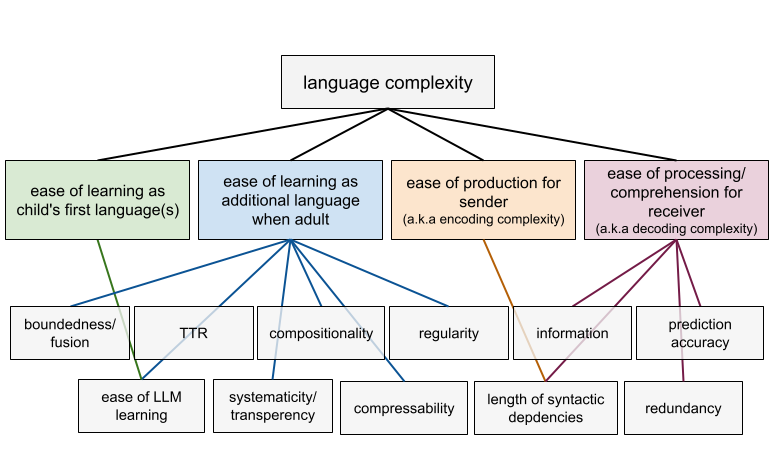
\includegraphics[width=0.9\textwidth]{latex/graphics/ud_complexity_metrics.png} % Change filename and width as needed
    \caption{Methods of quantifying language complexity, and their possible relationships with four overarching aspects which are typically not directly measured.}
    \label{fig:metrics_diagram}
\end{figure}
\FloatBarrier

The present study lays the ground for a wider investigation of how systematic pragmatic habits, over time and over language communities, can impact the structure of the language.
%%% SFM word chopping
% In particular, we are interested in informational distinctiveness, and the other side of the coin - ambiguity.
%%% SFM end word chopping
Several studies have sought to link sociocultural and demographic features with the various facets of linguistic complexity \citep{wray2007consequences,lupyan2010language,shcherbakova2023societies,levinson2024dark,dale_lupyan_2012}.
We are interested in exploring how systematic corpus-based cross-linguistic comparison can contribute to testing the strength of various hypotheses of this kind, especially those relating to pragmatics \citep{hall1976beyond,cardon2008critique,meyer2016culture}.
To that end, in this paper we define metrics of informational distinctiveness of morphological features based on datasets of the UD project. 

%%%%%%%%%%%%%%%%%%%%%%%%%%%%%%%%%%%%%
%%%%%%%%% SFM WORD CHOPPING %%%%%%%%%

% Is it the case that communities that tend to share a lot of common ground tend to create less informative utterances because the grammar of their languages makes fewer demands on informational distinctiveness?
% Scholars such as \citet{wray2007consequences} have suggested that communities with a lot of shared common ground develop less complex - specifically less compositional - languages due to constraints related to acquisition, conversational efficiency and processing. 
% This proposal has been tested in studies like \citet{lupyan2010language} and \citet{shcherbakova2023societies}, with contrasting results (possibly due to different samples, operationalisation of ``complexity'' and/or control for spatial and phylogenetic autocorrelation).
% We seek to explore the effect of pragmatic constraints on grammar, but contrary to \citet{wray2007consequences} consider informational distinctiveness instead of compositionality. 
% American anthropologist Edward Hall's has suggested that cultures of the world can be meaningfully understood on a dimension of ``high'' to ``low''-context communication styles \citep{hall1976beyond}.
% The high-context communicational style involves assuming a large degree of shared ground and context between interlocutors, whereas low-context involves presupposing  little shared information. 
% These pragmatic premises have consequences for the linguistic message. \citep[79]{hall1976beyond} writes: 
% \begin{quote}
% A high-context (HC) communication or message is one in which most of the information is either in the physical context or internalized in the person, while very little is in the coded, explicit, transmitted part of the message.
% A low-context (LC) communication is just the opposite; i.e., the mass of the information is vested in the explicit code.
% \end{quote}
% It is possible that communities that use HC messages more often end up with not only overall less information in their utterances (cf. ``leveraging context'' in \citet[29-31]{levinson2024dark}) - but perhaps also less information specified in the grammar of their languages.
% The second prediction follows on from the Linguistic Niche Hypothesis framework (LNH) \citep{dale_lupyan_2012} which proposes that the social context of learning and usage of a language may impact its structure.
% Hall's theory also connects the predominant communication style of a culture to the social heterogeneity, which can be compared to the connection between proportion of strangers/second-language speakers and various facets of ``complexity'' explored in the linguistics literature.
% Hall's theory of HC and LC communication has been widely applied and popular in Intercultural Business and Technical Communication \citep{meyer2016culture}.
% However, it has also been critiqued for not being empirically supported \citep{cardon2008critique}.
% We are interested in exploring how systematic corpus based cross-linguistic comparison can contribute to testing the strength of Hall's framework of cultural differences in communication styles as interpreted via LNH.
% To that end, in this paper we define metrics of informational distinctiveness of grammar (specifically morphological features) based on datasets of the UD project. 

%%%%%%% END SFM WORD CHOPPING %%%%%%%
%%%%%%%%%%%%%%%%%%%%%%%%%%%%%%%%%%%%%

%\citet{hall1976beyond}
% We are interested in variation in informational load of morphology as found in language use. 
% It is well-known that languages vary with regards to morphemes being phonologically bound to each other and how they form extensive paradigms. 
% We are interested not only in the existence of these informational structures but how they are utilised. 
% To that end, we investigate the information-theoretic measure of \textbf{surprisal} of morphological features in the cross-linguistic Universal Dependencies database \citep{UD_2.14}. 
% We are interested in exploring the connections between this topic and theories proposed by \citet{wray2007consequences, lupyan2010language} and \citet{hall1976beyond}. 
% However, for the study at hand we focus on the measurements themselves and comparisons with related measurements. 
% We have also included comparisons with population size of languages, but this is merely to give indication of the context of the different measurements. 
% For a thorough examination of the relationships between these metrics of `language complexity' and social conditions, more extensive analysis is necessary.

%In this paper, we are primarily interested in the pragmatics of information transfer between adult native speakers and how the trade-off between the encoding and decoding cost is balanced in different languages. Specifically, we are interested in how languages vary with respect to morphological information.


\FloatBarrier
\section{Study outline}
We aim to quantify the information in morphology annotations in corpora as a way of assessing how much information languages typically encode.
On this definition, an increase in morphological information can be understood as decreasing the ease of production for the sender, and thereby increasing one facet of `language complexity'.

Many corpora collections, such as the Universal Dependencies datasets v2.14 \citep{UD_2.14} which are used here, contain information on the morphology of individual words. 
Table \ref{tab:turkish_example} is an example of a sentence in Turkish where words are marked for the morphological categories case, number, person, aspect and more \citep{kuzgun_2020_UD_turkish_penn}.
%For example, the word ``horses'' in English would typically be tagged for the grammatical meaning ``plural'' being encoded morphologically.

\begin{table}[h]
    \centering
    \caption{Sentence 15-0000 from Universal Dependencies dataset Turkish-Penn \citep{kuzgun_2020_UD_turkish_penn}. UPOS : Universal Part-of-Speech, lemma = base form, token = specific word, feats = morphological features} %note table captions go above the table
    \label{tab:turkish_example}   
    \begin{tabular}{p{1.5cm}p{2cm}p{2cm}p{5cm}}
\toprule
	\textbf{UPOS}	&	\textbf{lemma}	&	\textbf{token}	&	\textbf{feats}	\\
    \midrule
	ADJ	&	devasa	&	Devasa	&	\\    \midrule
	ADJ	&	ölçek	&	ölçekli	&\\    \midrule
ADJ	&	yeni	&	yeni	&		\\    \midrule
	NOUN	&	kanun	&	kanunda	&	Case=Loc|Number=Sing|Person=3	\\    \midrule
	ADJ	&	kullan	&	kullanılan	&		\\    \midrule
ADJ	&	karmaşık	&	karmaşık	&\\    \midrule
CCONJ	&	ve	&	ve	&		\\    \midrule
ADJ	&	çetrefil	&	çetrefilli	&		\\    \midrule
	NOUN	&	dil	&	dil	&	Case=Nom|Number=Sing|Person=3	\\    \midrule
	NOUN	&	kavga	&	kavgayı	&	Case=Acc|Number=Sing|Person=3	\\    \midrule
	VERB	&	bulan	&	bulandırdı	&	Aspect=Perf|Mood=Ind|Number=Sing| Person=3|Polarity=Pos|Tense=Past| VerbForm=Fin|Voice=Cau	\\\midrule
   \multicolumn{4}{p{11cm}}{Translation: \textit{The complex and complicated language in the massive new law has muddied the fight.}}\\    \bottomrule
    \end{tabular}
\end{table}

In this study, we are not only interested in how many morphological features on average a token in a given language has, but also how informative those features are given their \textbf{lemma} or base form. 
%If tokens with the lemma ``kanun'' almost always has the value singular for the morphological feature category number, perhaps number is not so informative for those tokens?
Words in any language can be grouped according to their lemma. 
For example ``horse'', ``horses'', ``horse's (possessive)'' all have the same lemma, usually represented in the singular, nominative non-possessive form, i.e. ``horse''.
The information stored in the morphological feature on the token can be understood as dependent on the relative frequencies of that feature on that lemma. 

For example, in the Turkish-Penn dataset of Universal Dependencies 2.14 there are 52 tokens with the lemma ``kanun'' (Eng: \textit{law}).
Of these, 47 are marked as singular for the number category, and five as plural; most of the time when people use this word in this corpus, it's singular.
Were we only to know that a token belongs to the lemma ``kanun'', we would have a good chance (around 90\%) to guess correctly if we said it was in the singular form.
Intuitively, the category of number for this lemma is not very informative.
On the other hand, if we were to see an instance of a token with the lemma ``kanun'' with plural marking, we ought to be a bit more surprised.
By contrast, tokens for the lemma ``fiyat'' (Eng: \textit{price}) have a 55\%/45\% chance of being plural vs. singular (plural = 237, singular = 196). 
Were we to only know that a token was of this lemma, we'd have a harder time guessing its number category. 
The number morphology for ``fiyat'' is more informative than that for ``kanun''.
This intuition lies behind the information-theoretic measures defined in this paper.
We provide a quantitative answer to the question: how informative is the morphology of a particular language?

\subsection{Data}
We use Universal Dependencies (UD) v2.14 \citep{UD_2.14}, Grambank v1.0 \citep{grambank_release, grambank_dataset_zenodo_v1} and Glottolog v5.0 \citep{glottolog5.0}.
We also include population size data from Google's research team \citep{ritchie-etal-2024-linguameta-unified}.
We omit 22 UD datasets which lack any morphological feature annotations, as well as three multilingual datasets which would obscure language-specific metrics.

\subsection{Similar studies}
% There are a few studies that describe metrics of complexity similar to our study. 
\cite{grambank_release} and \citet{shcherbakova2023societies} both use measurements based on typological data from the Grambank dataset: Fusion (out of all Grambank features that target bound morphology, what proportion are answered positively?) and Informativity (out of all Grambank features which target if a grammatical distinction is made, how many are answered yes?\footnote{Unfortunately, the term ``informativity'' is found in the literature with at least two senses: how many grammatical distinctions a grammar makes possible \citep{shcherbakova2023societies, grambank_release} and the average contextual unpredictability \citep{cohen2008phone}. These two senses are distinct. When we refer to the Grambank informativity metric, we refer to the first one.}$^{,}$\footnote{For more details on these metrics, please see \citet{grambank_release} and \citet{R-rgrambank}.}). These metrics differ from the study at hand in that they describe the possibilities that the grammar of a certain language contains (as found in grammatical descriptions) rather than language usage (such as can be measured in corpora). 
We include these two metrics in our results section for comparison with the measures defined here. 
We use the R-package rgrambank to derive the Grambank metrics \citep{R-rgrambank}; see appendix \ref{sec:appendix_rgrambank} for details.
%%% SFM word chopping: moved to appendix
% \footnote{The calculation of Fusion and Informativity from raw Grambank data is somewhat involved. We combine dialects into languages, and if two dialects under the same language have different values for the same feature, we choose one at random. 
% We remove languages with more than 25\% missing data across the features used to calculate each metric. 
% We do this using the functions from the package rgrambank \citep{R-rgrambank}. 
% This data wrangling procedure differs slightly from \citet{grambank_release} and \citet{shcherbakova2023societies}, but the difference is negligible. 
% See example scripts accompanying the R-package rgrambank for illustration of procedure and differences. Unlike \cite{shcherbakova2023societies}, but like \cite{grambank_release} we use the version of the Grambank metric Fusion which awards features that cover bound morphology and other morphology half a Fusion-point.} 
%% SFM end word chopping

A recent study from \citet{ccoltekin2023complexity} also uses information theory to investigate corpus data from UD. 
Due to similarities with our own approach, we describe this metric in more detail in appendix \ref{sec:appendix_ccoltekin}.
Çöltekin \& Rama's goal is to determine the extent to which different measures of complexity latch onto the same underlying properties of a language. 
They analyse eight measures, from a simple count of the type/token ratio to the far more involved assessment of how accurately a machine learning model can predict an inflected word from its lemma and morphological features.
The measure most relevant for our purposes is \textbf{morphological feature entropy}, which captures how evenly spread morphological features are throughout a corpus.
This `even-spreadedness' connects to complexity in the manner outlined above: if there are many different features that have roughly similar frequency, it would be difficult to predict from a lemma alone what its features are; on the other hand if a few well-represented features dominate the corpus, a given lemma's features are likely to be more predictable.
Since predictability is intuitively connected to complexity, the even-spreadedness of morphological features in a corpus can indicate the complexity of a language.
This metric of Çöltekin \& Rama has since been used in further studies, such as \citet{bentz2023complexity}.

%%%%%%%%%%%%%%%%%%%%%%%%%%%%%%%%%%%%%%%%%%
%%%%% SFM: Below moved to appendix %%%%%%%

% The canonical mathematical way to measure this `even-spreadedness' is entropy.
% Defined as $\Sigma p \log{\frac{1}{p}}$ for probabilities $p$ of a given distribution, entropy is large when probabilities are more evenly distributed and small when a few probabilities are much greater than the others.
% Thus entropy captures something like the average amount of uncertainty among a set of items.
% Çöltekin \& Rama thus define a measure of the entropy of all morphological features in a dataset to capture one aspect of a language's complexity.
% Their method of calculating this value is as follows:\footnote{This procedure describes the code which can be found at \url{https://github.com/coltekin/mcomplexity/blob/main/mlc-morph.py}, specifically the method \texttt{get\_mfh}.} %We are grateful to Çöltekin \& Rama for corresponding with us so that we could confirm our understanding of their procedure. Any remaining misunderstandings are our own.}:
% \begin{enumerate}
% \item For a given dataset, randomly sample a fixed number of tokens
% \item Remove punctuation (UPOS=`PUNCT') and unanalysable tokens (UPOS=`X')
% \item Remove tokens that have no morphological features
% \item Split the remaining tokens' morphological features into a list (e.g. Table \ref{tab:mfh} lists the individual features in the sample shown in Table \ref{tab:turkish_example})
% \item Count how many times each feature occurs in the sample (column `Count' in Table \ref{tab:mfh})
% \item Calculate the relative frequency of each feature (column `Frequency (p)' in Table \ref{tab:mfh}; this is the feature's Count value divided by the sum of the Count column for the entire sample)
% \item Calculate entropy from the frequencies ($\Sigma p \log{\frac{1}{p}}$)
% \item Run steps 2-7 multiple times for different samples of the same size and take the mean entropy.
% \end{enumerate}

% \noindent Table \ref{tab:mfh} shows the components of the entropy measure for the sample of tokens listed in Table \ref{tab:turkish_example}.
% The total entropy for this sample is approximately 3.15 bits.
% In their study \citet{ccoltekin2023complexity} would sample something like 1000 tokens at a time, generating an entropy measure each time and then taking the average.
% This average is then an estimate of the `overall' entropy measure for the dataset.

% \begin{table}[h]
%     \centering
%     \caption{Components of the measure of morphological feature entropy as defined by \citet{ccoltekin2023complexity} for the sample of tokens in Table \ref{tab:turkish_example}. The total feature count is 17, and each feature's Frequency is its Count divided by this total (rounded to three significant figures). The entropy of this sample is 3.15 bits (also to three significant figures).} %note table captions go above the table
%     \label{tab:mfh}   
%     \begin{tabular}{p{5cm}p{3cm}p{3cm}}
% \toprule
% 	\textbf{Morphological feature}	&	\textbf{Count}	&	\textbf{Frequency (p)}	\\
%     \midrule
% 	Case=Loc&1&0.0588       \\    \midrule
% 	Number=Sing&4&0.235    \\    \midrule
%         Person=3&4&0.235		   \\    \midrule
% 	Case=Nom&1&0.0588	       \\    \midrule
% 	Case=Acc&1&0.0588		      \\    \midrule
%         Aspect=Perf&1&0.0588      \\    \midrule
%         Mood=Ind&1&0.0588		   \\    \midrule
%         Polarity=Pos&1&0.0588		\\    \midrule
% 	Tense=Past&1&0.0588	     \\    \midrule
% 	VerbForm=Fin&1&0.0588	    \\    \midrule
% 	Voice=Cau&1&0.0588      	\\ \bottomrule

%     \end{tabular}
% \end{table}


%%%%% SFM: Above moved to appendix %%%%%%%
%%%%%%%%%%%%%%%%%%%%%%%%%%%%%%%%%%%%%%%%%%

A similar measure was previously defined by \citet{SPROAT14.47}.
Their focus is on the popular question of which language is the most efficient, which they interpret as packing the most information into the shortest space.
They discuss different methods of quantifying both `information' and `space' in order to obtain ratios $\frac{\text{information}}{\text{space}}$ for different languages.
One of their measures of information weights words by the \textbf{surprisal} of their morphological features.
The surprisal of an event is a function of its probability: it is the logarithm of the reciprocal, written $\log{\frac{1}{p}}$, so that events with lower probability have higher surprisal.
\citet{SPROAT14.47} obtain these probabilities by estimating them; however, they do not fully describe how the estimate is produced.
They use customised feature annotations rather than Universal Dependencies datasets, and they report results for only eight languages and fewer than 1,000 sentences per language.
Their work can therefore be seen as a step towards the kind of measure defined by \citet{ccoltekin2023complexity} as well as our own; however, their relatively small sample size suggests that quantitative comparison with our results would not be particularly enlightening.

\subsection{Overview of our metrics}
\label{detailed_procedure}
Çöltekin \& Rama use entropy as their measure.
Technically entropy is itself the average surprisal of all events in an entire distribution.
%%% SFM word chopping
% Each row in Table \ref{tab:mfh} therefore has its own surprisal, and it is the average of these that constitutes the entropy.
%%% End SFM word chopping
Our metric also uses surprisal as the basis of a measure of complexity.
However, instead of entropy, we define measures of \textbf{mean surprisal per token}.
As noted above, calculating the morphological surprisal of a token requires calculating the probabilities of its morphological features.
Whereas \citet{ccoltekin2023complexity} calculate frequencies on a sample-by-sample basis, and \citet{SPROAT14.47} estimate frequencies in an unknown manner, we calculate frequencies across the entire corpus for each UD dataset.
The full procedure of our basic metric can be found in appendix \ref{sec:appendix_ours}.

%%%%%%%%%%%%%%%%%%%%%%%%%%%%%%%%%%%
%%% SFM below moved to appendix %%%

% The full procedure of our basic metric is as follows:
% \begin{enumerate}
% \item Combine the files of each UD dataset (e.g. dev, test and train) to one table with one token per row
% \item Remove punctuation (UPOS=`PUNCT'), symbols (UPOS=`SYM') and unanalysable tokens (UPOS=`X')
% \item Define lemmas as a combination of lemma + UPOS, so that lemmas that are spelled the same but belong to different UPOS can be distinguished. \textit{Example:} the noun ``mark'' and the verb ``mark'' in English are defined as having the lemmas ``mark\_NOUN'' and ``mark\_VERB'' as opposed to both potentially being assigned to the same lemma ``mark''.
% \item Determine the full set of morphological feature categories per lemma. \textit{Example:} the token `sebuah' in Table \ref{tab:unassigned_ex} has features Definite and PronType; supposing there were another token of the same lemma in the dataset that had a value for the category Number, then the full set of categories for `sebuah' would be Definite, Number and PronType.
% \item Remove features that are not related to morphology: ``Abbr'' (abbreviations), ``Typo'' (whether or not a token has a typo) and ``Foreign'' (whether or not a token is deemed as in a foreign language)
% \item Assign a dummy value to unassigned morphological categories for each token, given the other available feature categories for tokens of the same lemma. \textit{Example:} for `sebuah' we insert the dummy feature Number=unassigned.
% \item Split the tokens' morphological features into a list (e.g. Table \ref{tab:unassigned_ex_SPLIT} lists the individual features for the sample shown in Table \ref{tab:unassigned_ex})\footnote{Some tokens have been given more than one feature value for the same feature category. This is allowable within the UD-framework, though the coordinators note that such multi-values should be used sparingly. For example, the adjective ``{\dolousfont ἀ}{\Timesfont όρατος}'' in the Ancient Greek PTNK-dataset is assigned ``Gender=Fem,Masc''. We are treating instances like these as a case of the feature value being ``Fem,Masc'' and not a case of both ``Gender=Fem'' and ``Gender=Masc''.}
% \item Count how many times each feature \textit{value} occurs \textit{for that category, in tokens of that lemma} (column `Count' in Table \ref{tab:unassigned_ex_SPLIT})
% \item Calculate the relative frequency of each feature value (column `Frequency' in Table \ref{tab:unassigned_ex_SPLIT}; this is the feature value's Count divided by the number of times that lemma appears in the dataset)
% \item Calculate the surprisal of that feature value for that token: $\log{\frac{1}{\text{frequency}}}$
% \item Calculate the total `surprisal of a token' by summing the surprisals of all its features (including dummy-assigned features)

% % \item Calculate the mean surprisal in the dataset by summing the surprisals and dividing by the number of tokens.
% \end{enumerate}

% \begin{table}[h]
%     \centering
%     \caption{Four tokens from the treebank UD\_Indonesian-PUD. The token `sebuah' has no feature value for Number, but in this illustrative example we imagine that other tokens of the same lemma do have this feature. We therefore include it as an unassigned feature; likewise for `para' and the feature Definite. Of the adjectives, neither `baru' nor `terakhir' have a value for the feature NumType; we continue to imagine that there is at least one lemma for each of these tokens that does have a value for this feature, therefore both are given it as an unassigned feature. In fact the token `baru' has no feature values of its own; thus it takes all features possessed by any other token of the lemma `baru' as unassigned.} %note table captions go above the table
%     \label{tab:unassigned_ex}   
%     \begin{tabular}{p{1cm}p{1.4cm}p{1.5cm}p{3.5cm}p{2.5cm}}
% \toprule

% % UD\_Indonesian-PUD
% %id	&
% UPOS&lemma	&token	&feats & unassigned feats	\\ 
% \midrule
% DET & buah & sebuah 
% & Definite=Ind|PronType=Art
% & Number
% \\\midrule
% DET & para	& para	&Number=Plur|PronType=Ind & Definite
% \\\midrule
% ADJ&baru	&baru&
% & Degree \newline
% NumType 
% \\\midrule
% ADJ & akhir	&terakhir&	Degree=Sup& NumType\\\bottomrule
% \end{tabular}
% \end{table}

% % OUR APPROACH, FEATURES SPLIT
% \begin{table}[h]
%     \centering
%     \caption{Four tokens from the treebank UD\_Indonesian-PUD. For illustrative purposes we imagine this dataset contains 20 occurrences of the lemma `buah', 10 of `para', 5 of `baru' and 12 of `akhir'. The Count and Frequency columns, whose values in this table are also illustrative and not real, answer the question: `how often does this lemma have this value for this feature?'. The frequencies are used to calculate the surprisal of a particular token. For example, the surprisal of the token `sebuah' is $\log{\frac{1}{0.3}}+\log{\frac{1}{0.05}}+\log{\frac{1}{0.5}} = 7.06\text{ bits}$ (to three significant figures).} %note table captions go above the table
%     \label{tab:unassigned_ex_SPLIT}   
%     \begin{tabular}{p{0.7cm}p{1cm}p{1.4cm}p{1.3cm}p{1.5cm}p{1.4cm}p{1.6cm}}
% \toprule

% %id	&
% UPOS&lemma	&token	&feat name & feat value & Count\newline (illustrative) & Frequency\newline (illustrative)	\\ \midrule

% DET & buah & sebuah & Definite& Ind & 6 & 0.3\\
% DET & buah & sebuah & Number& unassigned & 1 & 0.05\\
% DET & buah & sebuah & PronType& Art & 10 & 0.5
% \\\midrule
% DET & para	& para	&Definite & unassigned & 1 & 0.1\\
% DET & para	& para	&Number & Plur & 4 & 0.4\\
% DET & para	& para	&PronType & Ind & 6 & 0.6
% \\\midrule
% ADJ&baru	&baru& Degree&unassigned & 4 & 0.8\\
% ADJ&baru	&baru& NumType&unassigned & 1 & 0.2 \\\midrule
% ADJ & akhir	&terakhir&	Degree& Sup & 3 & 0.25\\
% ADJ & akhir	&terakhir&	NumType & unassigned & 4 & 0.333\\
% \bottomrule
% \end{tabular}
% \end{table}


%%% SFM above moved to appendix %%%
%%%%%%%%%%%%%%%%%%%%%%%%%%%%%%%%%%%

Our approach differs in several ways from that of Çöltekin \& Rama.
First, we do not omit tokens that have no morphological features.
Instead, we introduce a dummy feature value `unassigned' for those tokens that do not have an assigned value for each morphological feature associated with that token's lemma.
%%% SFM word chopping
% For example, the determiner token `para' in the dataset described by Table \ref{tab:unassigned_ex} has no morphological feature corresponding to the category Definite.
% Supposing another token of the same lemma does have a feature value for Definite in this dataset, we would add the dummy feature `Definite=unassigned' to this token.
%%% SFM end word chopping
In this way we ensure that we include unmarked tokens in our calculation of surprisal.
This is important: if (say) 99\% of tokens of a given lemma have no Definite marking and 1\% of them have Definite=Ind, possession of a Definite marker should count as very surprising.
Without the dummy assignment this fact would be lost: the 1\% of Definite=Ind tokens would all get a frequency of 1 (because that's the only value for that feature across that lemma) and a surprisal of zero (because $\log{\frac{1}{1}}=\log{1}=0$).

A second key difference with Çöltekin \& Rama is as follows.
Instead of calculating the average surprisal of features across the entire sample of tokens, we split features into their component category/value pairs, and calculate the sum of the surprisals of feature values for a given token.
This produces what might be thought of as `the surprisal of the token': the amount of information a token carries by virtue of its morphological feature markings or lack thereof.
Once we have a measure of surprisal per token, we can average this across the entire dataset to obtain mean surprisal per token.
This indicates `the surprisal of the language': how surprising tokens of this language tend to be.
If there are very many morphological features whose values are all somewhat evenly represented among the tokens of the dataset, mean surprisal will be high.
If on the other hand each lemma has only a few features, or if a small number of feature values are much more likely than others, mean surprisal will be small.

%%% SFM Chopping: moved to appendix
% Clearly our mean surprisal measure is capturing something similar to the classical entropy measure, but they are not strictly equivalent.
% Entropy weights surprisal by the same probability that defines the surprisal: the two $p$'s in the formula $\Sigma p\log{\frac{1}{p}}$ are the same.
% By contrast our measure calculates a sum of surprisals, each of which is defined in terms of the frequencies of its morphological feature values.
% Only then do we calculate a mean value by summing across the entire dataset.
% The formula describing our measure is therefore $\Sigma_i p_i \left( \Sigma_{j_i} \log{\frac{1}{p_{j_i}}} \right)$ where $i$ ranges across tokens and $j_i$ ranges across feature values of token $i$.
%%% SFM end chopping

There are several variants of this procedure, yielding slightly different measures of morphological information per dataset.
One variant aggregates features at the level of UPOS rather than lemma.
In this case tokens receive many more ``dummy'' unassigned feature values: all those categories that occur on any token of the same UPOS, which will generally be a longer list than just those that occur on tokens of the same lemma.
Another variant controls for variability in morphological feature annotations across datasets by using only the ``core'' features as defined by the UD project (see appendix \ref{caveat_comparability} for more).
A final variant treats the token's entire list of feature category-value pairs (after dummy value insertion) as the basis of the surprisal measure: only tokens with \textit{exactly the same} feature values get to count as `the same' for the purposes of calculating frequencies, hence surprisal.
We indicate this variant with the term `featstring', since the full list of features is concatenated into a single string before frequency calculation.

Overall, we define eight versions of our metric:

\begin{enumerate}
    \item \textbf{surprisal of morphological features per token}
    \begin{enumerate}
  \renewcommand{\labelenumi}{\alph{enumi})}
  \item \textbf{aggregation level}: lemma; \textbf{features:} all; \textbf{frequencies calculated over}: feature values
  \item lemma; core only; feature values
  \item UPOS; all; feature values
  \item UPOS; core only; feature values
  \item lemma; all; featstring
  \item lemma; core only; featstring
  \item UPOS; all; featstring
  \item UPOS; core only; featstring
\end{enumerate}
\end{enumerate}

We note caveats to our approach in appendix \ref{sec:caveats}. 

\subsection{Additional metrics}
We also calculate related metrics which are commonly reported in similar studies.
%Like for the metrics defined above, some of those listed here depend on whether the aggregation level is lemma or UPOS, and whether all features or only core features are considered.
\begin{enumerate}
  \setcounter{enumi}{1}  % This will start the list at 2
 %    \item Mean surprisal of morphological features when concatenated as a string, e.g. ``Number=Plur|PronType=Ind'' instead of split per feature and feature category versus feature value (see section \ref{caveat_conditional_order}). Labelled ``featstring'' in results plots. 
 %    \begin{enumerate}
 %    \renewcommand{\labelenumi}{\alph{enumi})}
 %  \item aggregation level = lemma, all features
 %  \item aggregation level = lemma, core features only
 %  \item aggregation level = UPOS, all features
 %  \item aggregation level = UPOS, core features only
 % \end{enumerate}
  \item Type-Token Ratio (TTR): the number of unique tokens divided by the total number of tokens
  \item Lemma-Token Ratio (LTR): the number of unique lemmas divided by the total number of tokens
  \item Mean number of morphological features per token (calculated before dummy features are inserted, so aggregation level is irrelevant)
      \begin{enumerate}
  \renewcommand{\labelenumi}{\alph{enumi})}
  \item all features
  \item core features only
 \end{enumerate}
   \item Mean token surprisal: mean surprisal per token given all tokens, regardless of UPOS/lemma or morphological features
\end{enumerate}

\noindent We also report some simple statistics for each dataset, namely:

\begin{enumerate}
  \setcounter{enumi}{9}  % This will start the list at 5
  \item Number of types
  \item Number of tokens
  \item Number of sentences
  \item Number of unique features% (comparable to Grambank metrics Fusion and Informativity)
      \begin{enumerate}
    \renewcommand{\labelenumi}{\alph{enumi})}
 \item  all features
  \item core features only
 \end{enumerate}
 \end{enumerate}

For comparison with information external to UD, we also include:

\begin{itemize}
    \item Grambank metrics (for detailed definitions see \citet{grambank_release}, \citet{shcherbakova2023societies} and \citet{R-rgrambank}) 
\begin{itemize}
\item Fusion 
\item Informativity 
\end{itemize}
    \item Speaker population estimates, compiled by Google's research team \citep{ritchie-etal-2024-linguameta-unified}
\end{itemize}


\section{Results}
We report the results in ScatterPlOt Matrices (SPLOMs) and maps.\footnote{Unfortunately there are no UD datasets present in the Americas or Central or Eastern Pacific, which is why these regions are not displayed on the maps. Furthermore, the geographical points are tied to the locations of the languages in Glottolog 5.0 \citep{glottolog5.0}. The points have been jittered somewhat to avoid overlaps which would obscure information.}
The SPLOM visualisations compare different measurements of the same data in a  pairwise fashion. 
The lower-left portion of each SPLOM shows scatterplots for the pairwise comparisons of measurements.
The upper-right portion shows the Pearson correlation coefficient of the corresponding pair. 
The diagonal of the plot shows histograms of each measure. 
The upper and right edges of the diagram list the names of each measure, while the left and lower edges display axis values for the scatterplots.

The Pearson correlation test evaluates the strength and significance of a linear relationship between two variables. 
The strength is expressed by a coefficient whose value lies between -1 (indicating negative correlation) and 1 (positive correlation). 
An absolute value of 1 indicates a perfect relationship in which the two variables are fully matched. 
Significance is measured via traditional p-values.
Significant correlations (p<0.05) are presented in bold text and marked with an asterisk. 
An absolute correlation coefficient larger than 0.6 is commonly interpreted as a strong relationship, and above 0.8 very strong. 
We have marked significant correlations above 0.6 in red text.
For each pair of measurements, we compare as many overlapping data-points as possible.
The number of data-points compared for each pair is reported in the upper triangle of the SPLOM as n.\footnote{When comparing between measurements based on the UD datasets, each point represents a single UD dataset. When comparing against the Grambank metrics Fusion and Informativity and Google's population numbers, the UD datasets are matched to entries in Grambank via glottocodes \citep{glottolog5.0} using the documentation of each dataset as a guide. When comparing between the Grambank metrics and Google's population data, the comparison is only made for unique pairs of glottocodes in order to avoid double-counting. We only compare data-points for which at least one UD dataset exists.}
In addition to the raw language speaker population numbers from the Google data, we also include a logarithmic transformation.
This makes comparison to other metrics easier and reduces the effect of outliers \citep{changyong2014log}.
%%% SFM word chopping: added to appendix
% Since the Google data lists two languages as having zero population, and the logarithm of zero is undefined, we add 1 to all population figures before the transformation.
% This has the undesirable consequence of treating extinct languages as though they have a very small number of speakers.
% However, the relationship between population size and language features is likely coarse at best, so grouping extinct languages with very small languages does not jeopardise the broad conclusions that can be drawn.
%%% SFM end word chopping.

UD datasets can vary considerably in terms of genre, which can have an impact on the measurements we are calculating. 
The UD datasets that belong to the Parallel Universal Dependencies (PUD) subset are more comparable in genre. 
Therefore, we report results both for all UD datasets and for the PUD datasets only. 
See Appendix section \ref{sec:caveat_genres} for more information.

\subsection{Custom metrics}

Firstly, we consider the relationship between the new metrics defined in this paper. 
Figures \ref{fig:SPLOM_custom_metrics} and \ref{fig:SPLOM_custom_metrics_PUD} show the relationship between the eight measurements we calculate, for all datasets and for PUD datasets only. 
% The measures are calculated separately for individual features and combinations of features (``featstring''), for aggregation levels UPOS and lemma, and with all features or just the core features.
% With three binary distinctions (feat vs featstring, UPOS vs lemma, core vs all features), we have eight different measures. 
Most of these correlate strongly with each other, suggesting that while they differ in specific implementation they are picking up on the same characteristics of the datasets (and thereby languages) in question. 
The correlations are even stronger if we consider only the PUD-subset of UD (Figure \ref{fig:SPLOM_custom_metrics_PUD}), indicating that the variation among the full complement of datasets is partly due to genre.


\begin{figure}
    \centering
    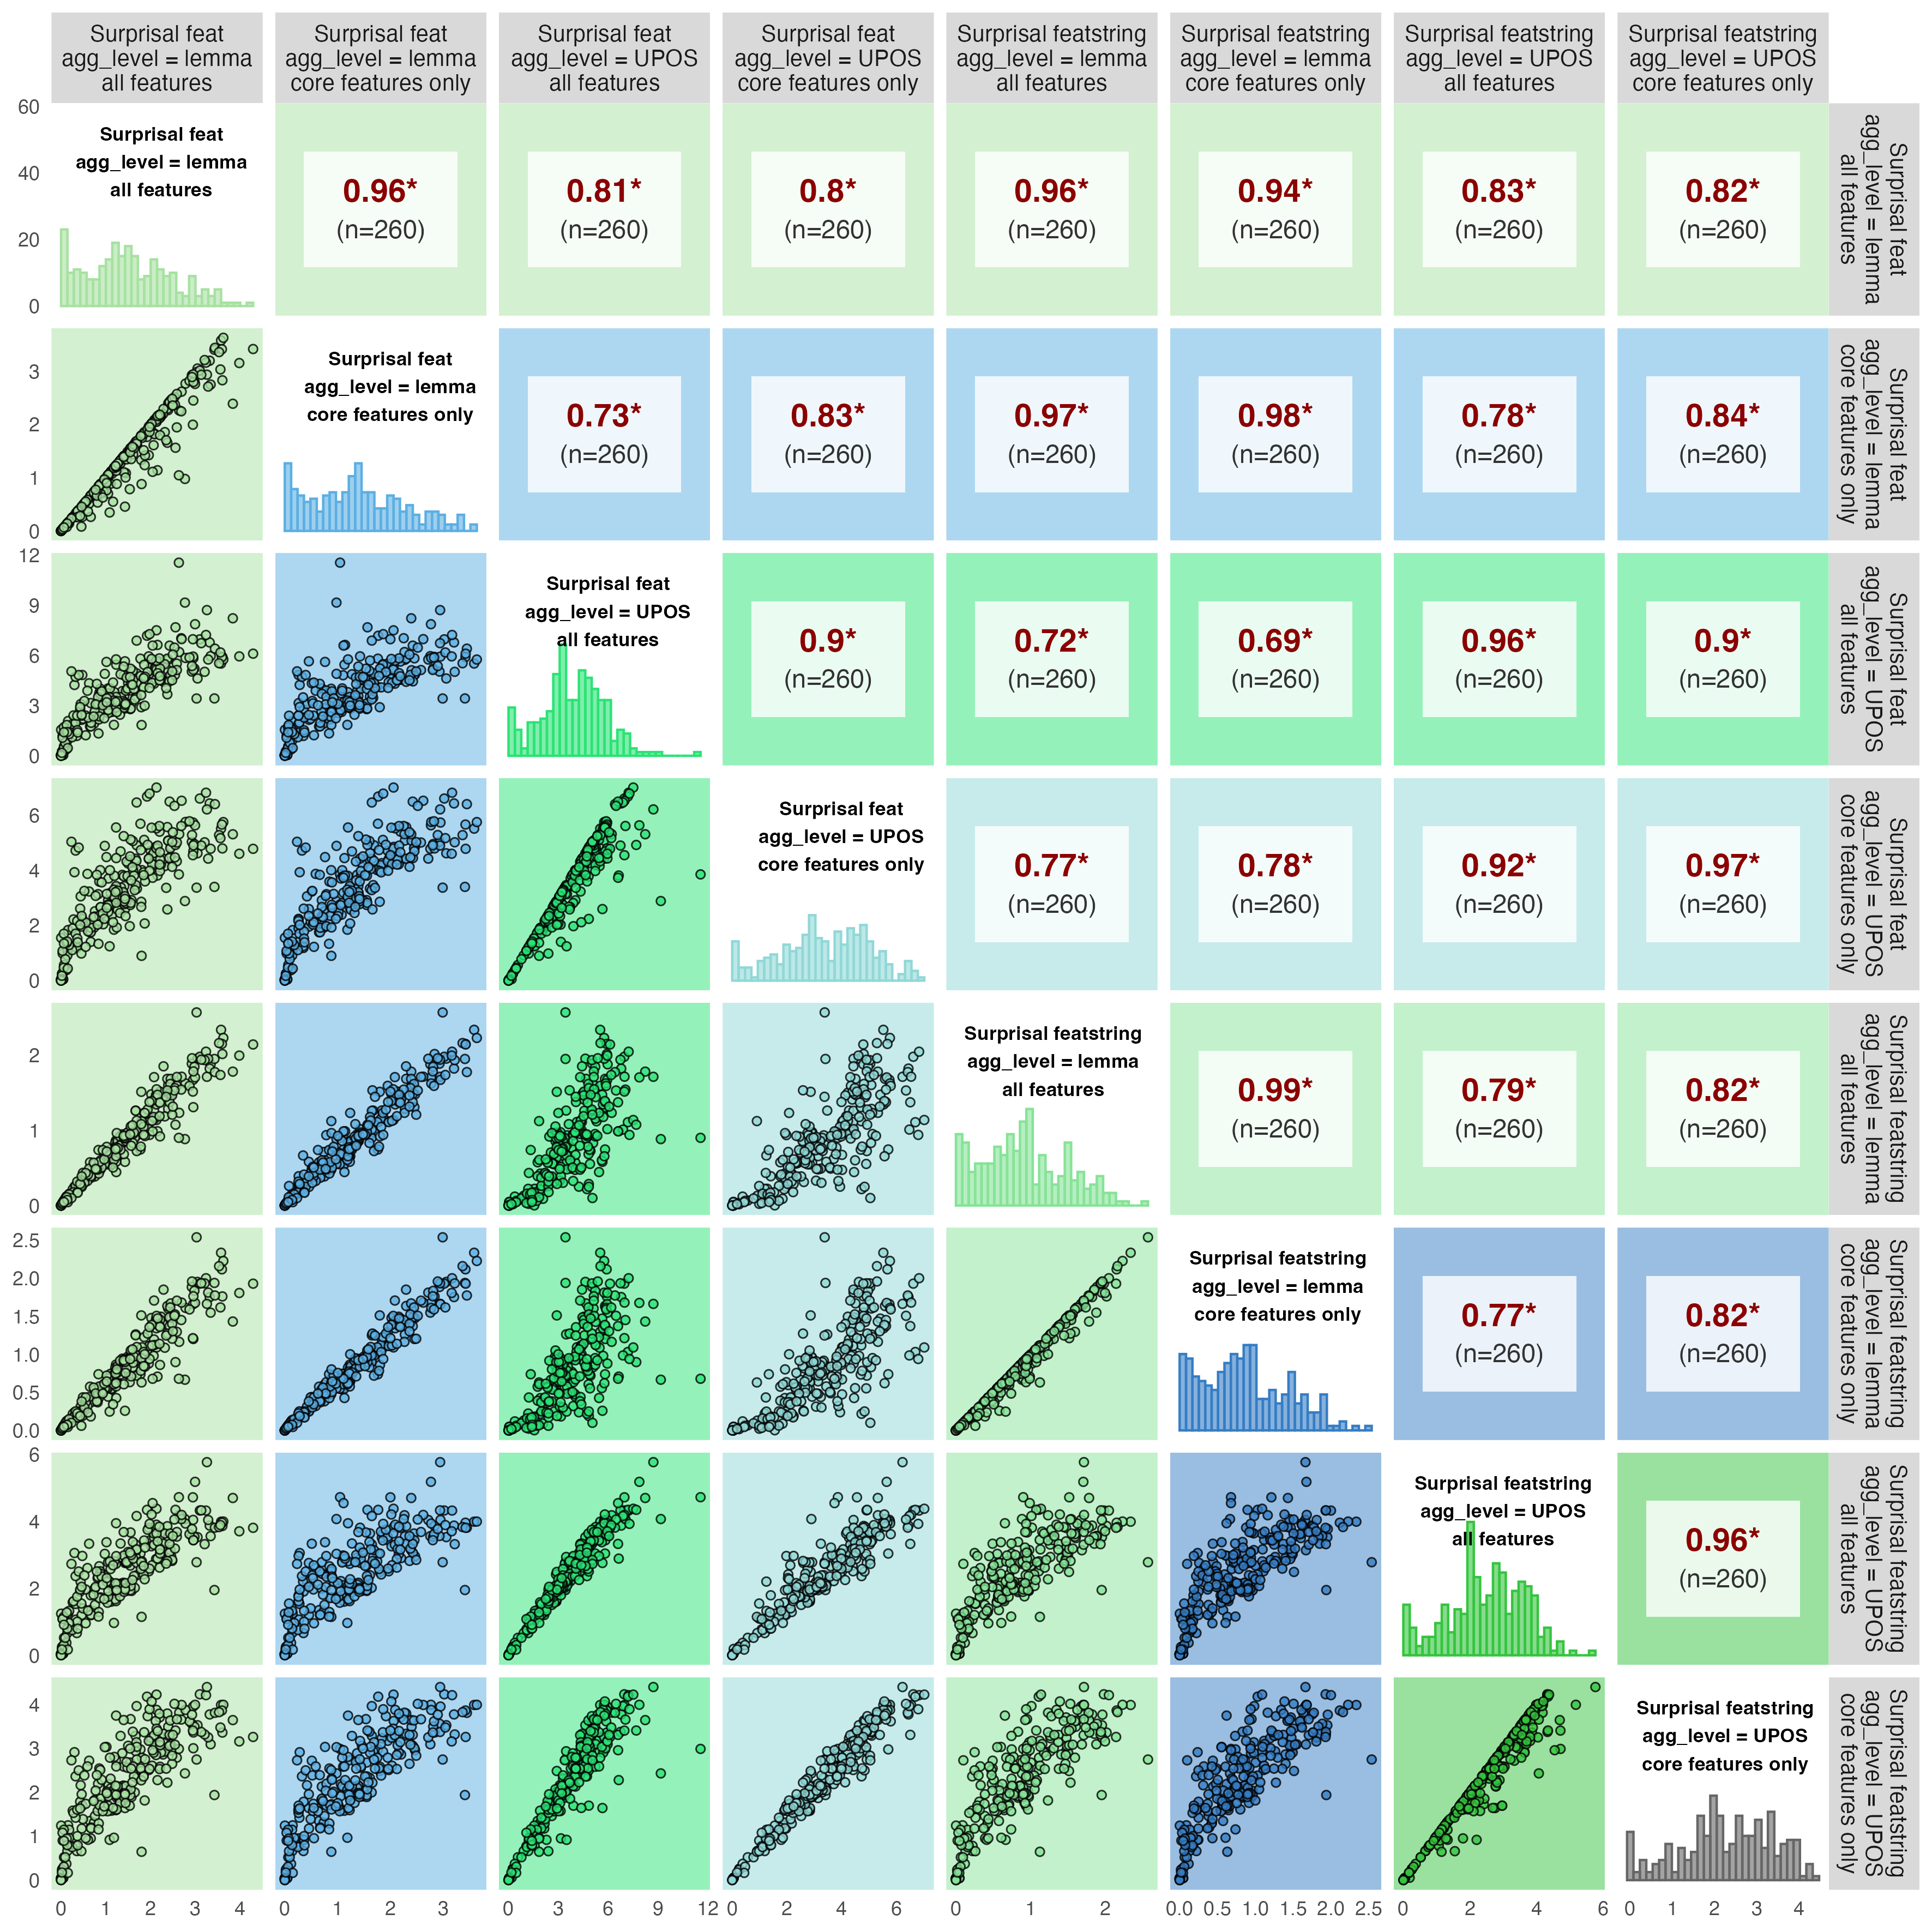
\includegraphics[width=1\linewidth]{latex/graphics/SPLOM_custom_metrics.png}
    \caption{SPLOM of custom metrics (all UD datasets). Since all eight measures are variations on the theme `mean surprisal per token', the correlations are all strong or very strong. The third and sixth measures here are used for comparison with other metrics in Figures \ref{fig:SPLOM_other_metrics} and \ref{fig:SPLOM_metrics_external}.}
    \label{fig:SPLOM_custom_metrics}
\end{figure}

\begin{figure}
    \centering
    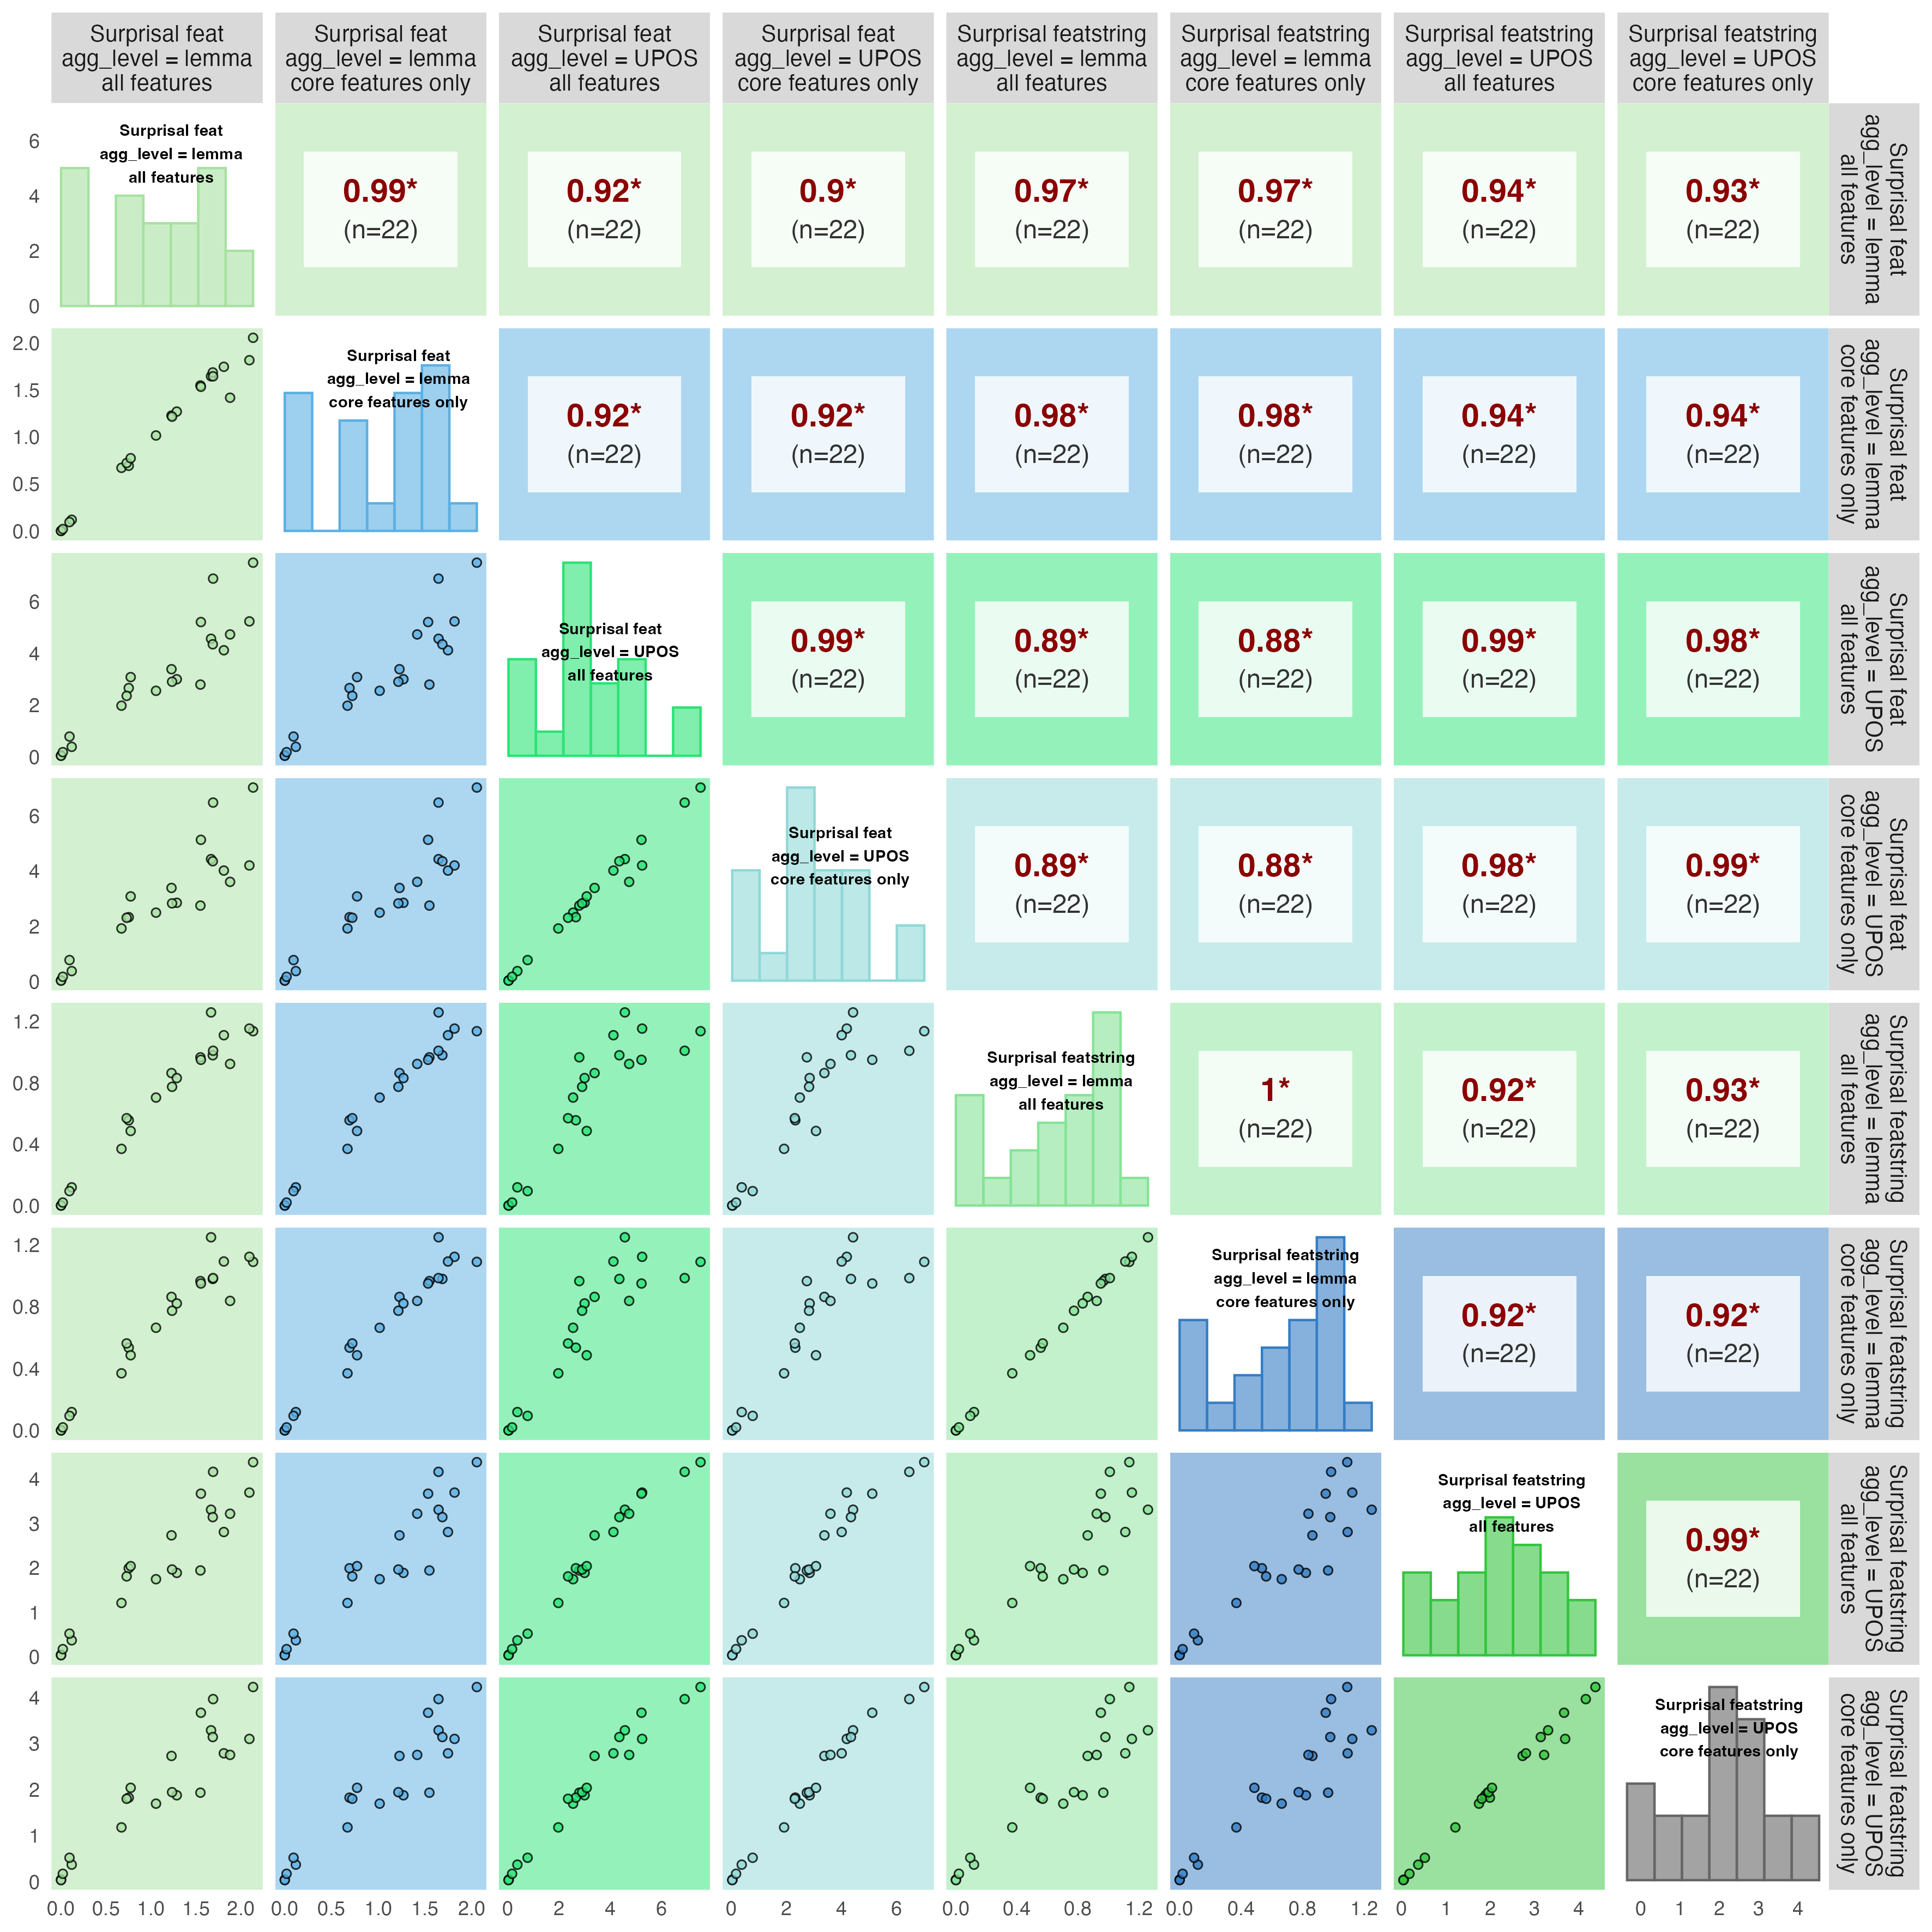
\includegraphics[width=1\linewidth]{latex/graphics/SPLOM_custom_metrics_PUD.png}
    \caption{SPLOM of custom metrics (PUD datasets only). Since the PUD datasets are smaller in size and uniform in genre, the correlations are stronger than their counterparts in Figure \ref{fig:SPLOM_custom_metrics}. The third and sixth measures here are used for comparison with other metrics in Figures \ref{fig:SPLOM_other_metrics_PUD} and \ref{fig:SPLOM_metrics_external_PUD}.}
    \label{fig:SPLOM_custom_metrics_PUD}
\end{figure}

\FloatBarrier
\noindent The two custom metrics that differ the most from each other are:
\begin{itemize}
    \item Mean sum surprisal of features, aggregation level = UPOS, all features (Figure \ref{fig:map_sum_surprisal_morph_split_mean_upos_all_features})
    \item Mean sum surprisal of featstring, aggregation level = lemma, core features only (Figure \ref{fig:map_surprisal_per_morph_featstring_mean_lemma_core_features_only})
\end{itemize}

Therefore, we will include these two in further plots as they represent the variation of our custom metrics. 
Their definitions are also complementary (features vs featstring, UPOS vs lemma, all features vs core only), so it makes sense that they would correlate the least with each other.
Figure \ref{fig:maps_custom_two} shows the distribution of these two metrics across the datasets linked to language locations. 
These distributions are similar to the morphological patterns of isolating/aggulinating/fusional languages often referenced in linguistic typology (cf. \cite{comrie1989language} and \cite{william1990typology}), with `hot spots' in eastern Europe and Central Asia and lower values in Southeast Asia. 
However, as several key areas are missing or severely under-represented (primarily the Americas and Australia), the seeming alignment of our values with patterns discussed in the literature is indicative rather than conclusive.


\begin{figure}[htbp]
  \centering
  \subfigure[Mean sum surprisal of features (in bits), aggregation level = UPOS, all features\label{fig:map_sum_surprisal_morph_split_mean_upos_all_features}]{
    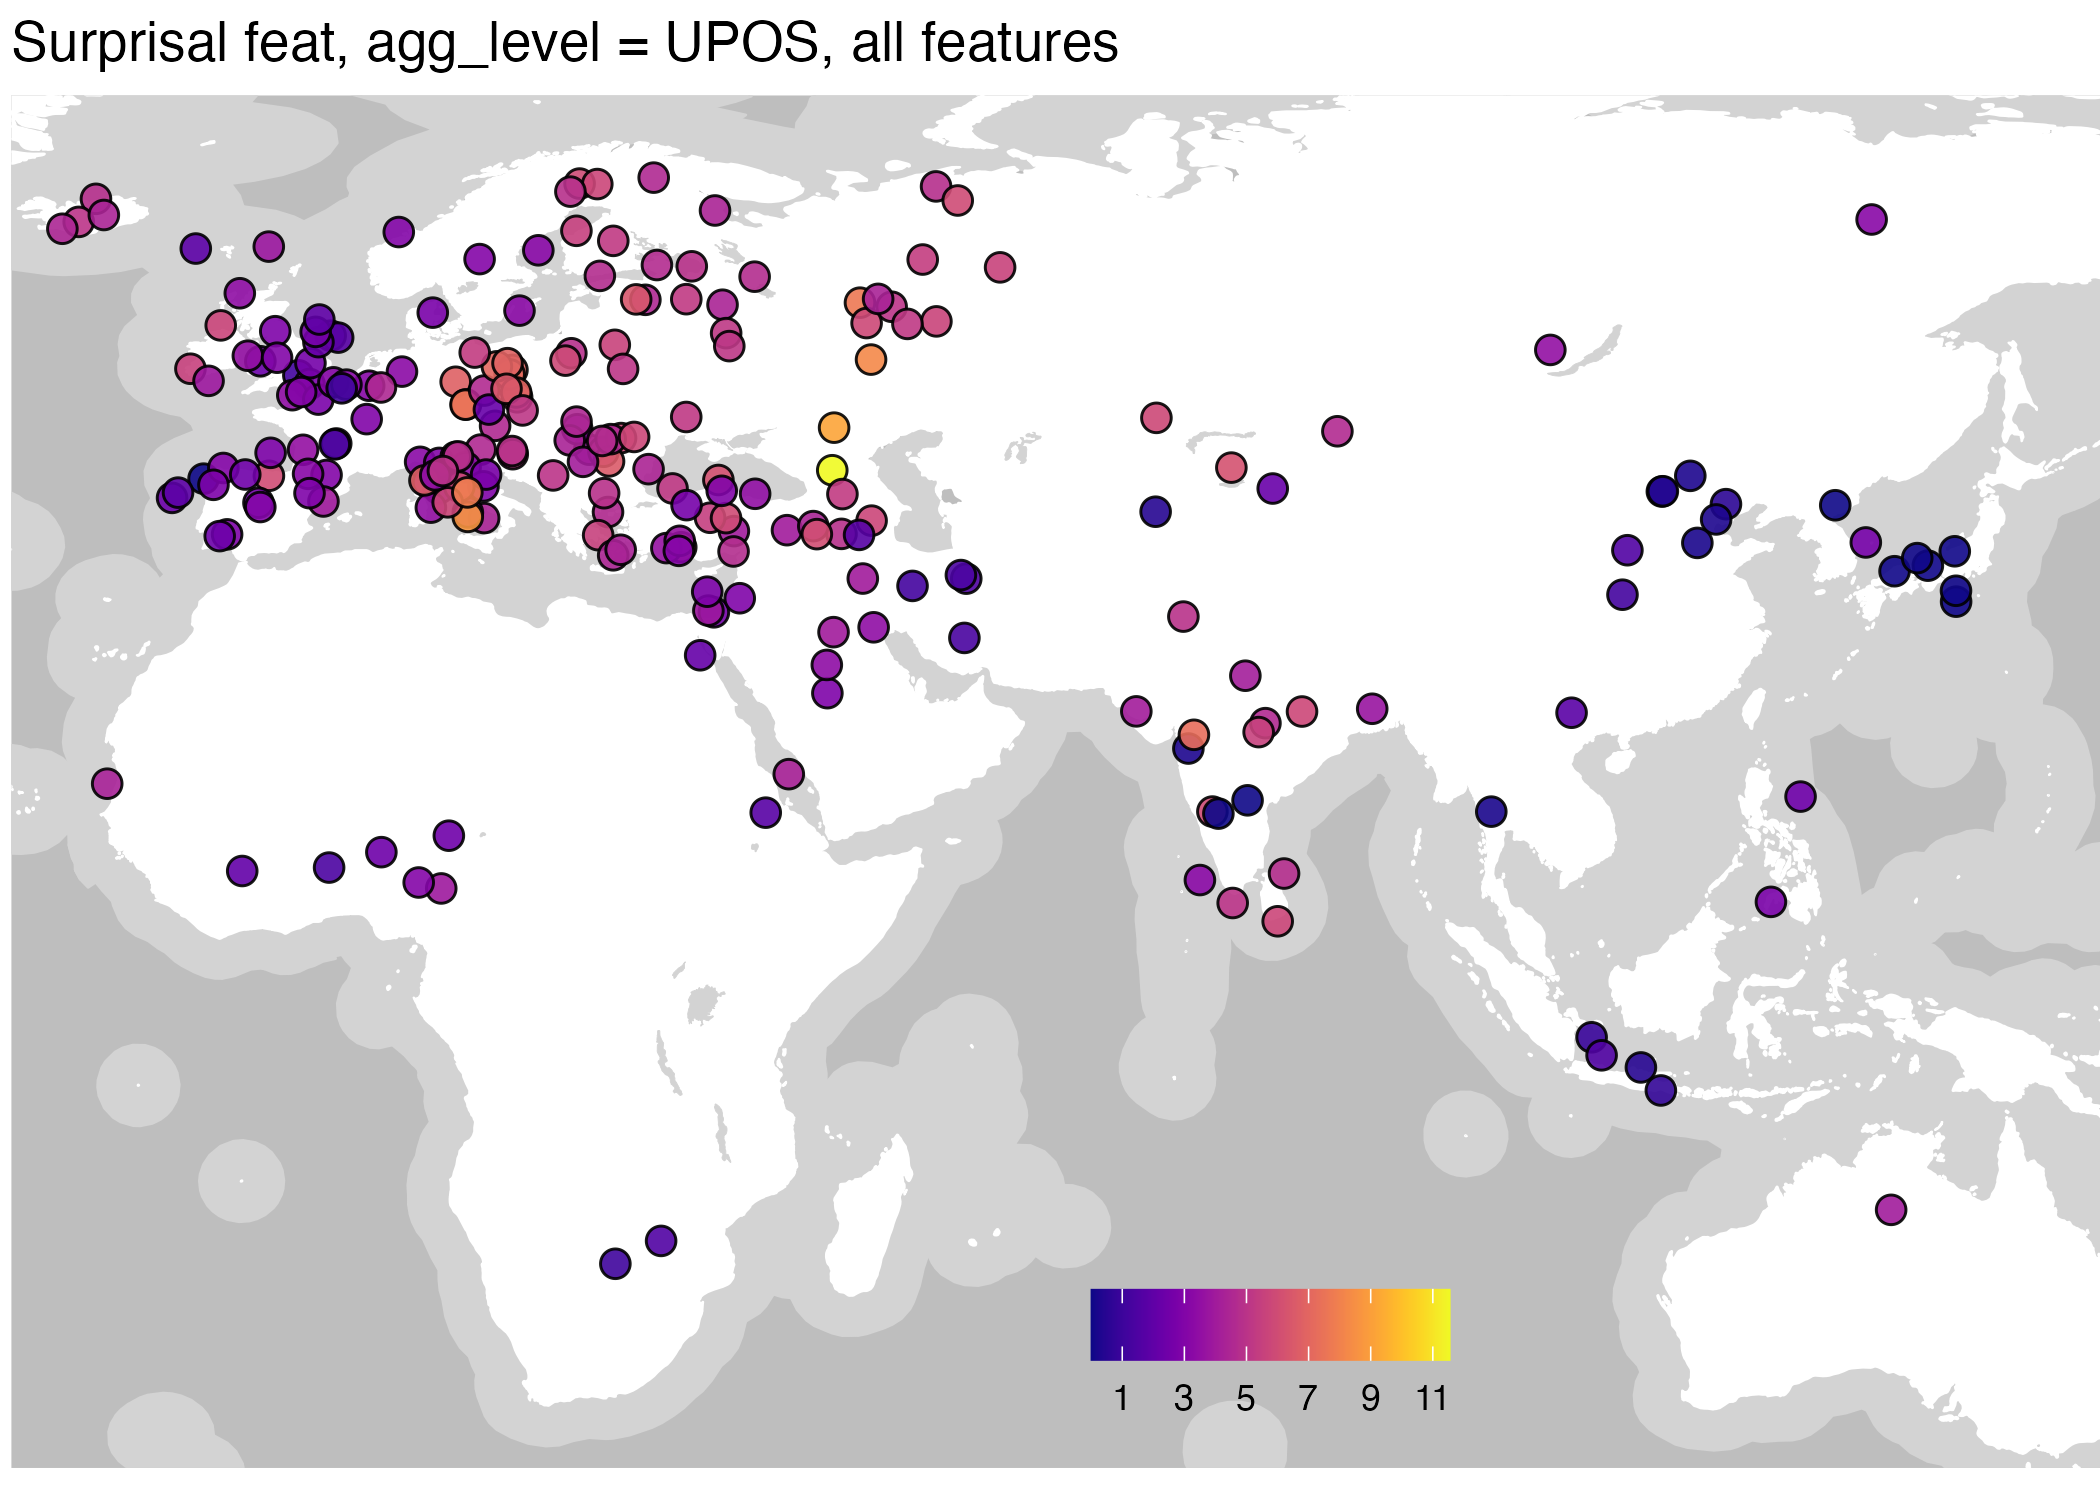
\includegraphics[width=0.45\linewidth]{latex/graphics/map_sum_surprisal_morph_split_mean_upos_all_features.png}
  }
  \hfill
  \subfigure[Mean sum surprisal of featstring (in bits), aggregation level = lemma, core features only\label{fig:map_surprisal_per_morph_featstring_mean_lemma_core_features_only}]{
    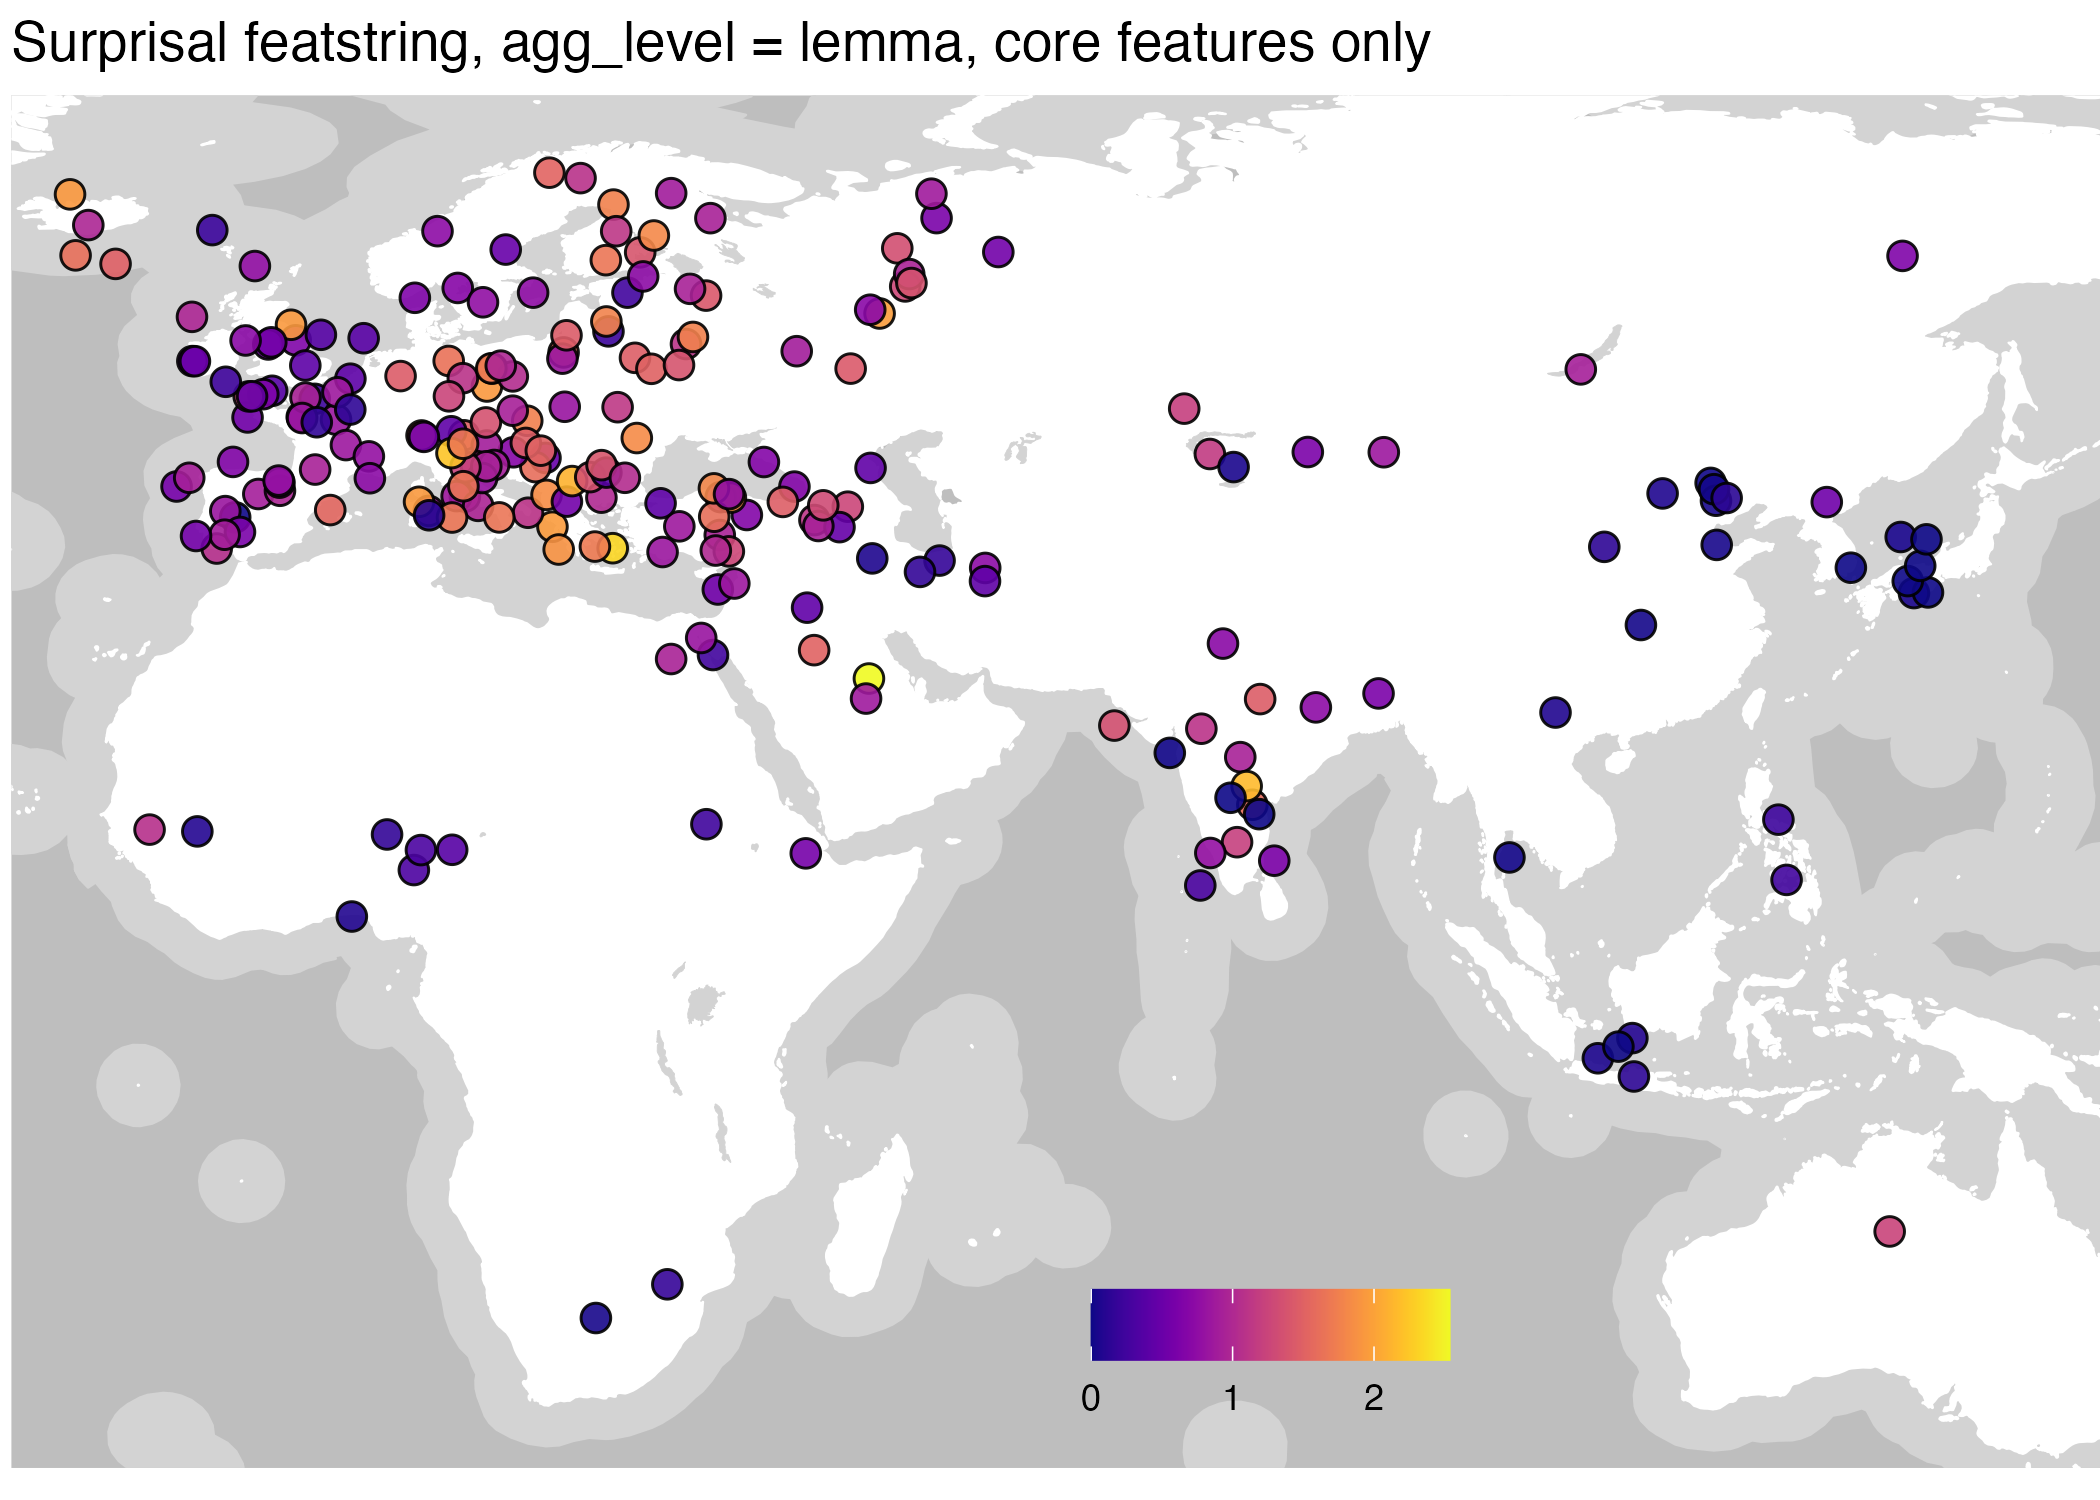
\includegraphics[width=0.45\linewidth]{latex/graphics/map_surprisal_per_morph_featstring_mean_lemma_core_features_only.png}
  }
  \caption{Maps showing two of the custom metrics.}
  \label{fig:maps_custom_two}
\end{figure}

\subsection{Other UD metrics}

Secondly, we compare our custom metrics to other metrics and statistics calculable from UD datasets in Figures \ref{fig:SPLOM_other_metrics} (all datasets) and \ref{fig:SPLOM_other_metrics_PUD} (PUD datasets only).
In these figures, the two representatives from our set of custom metrics appear first, as the green and blue rows/columns at the upper left of the plot.
As expected, the \textbf{mean number of features per token} correlates with both of our custom metrics: more features entails a lower frequency per feature, which translates directly to higher surprisal.
We also see a strong correlation between our UPOS-level metric and the \textbf{total number of feature categories} in the datasets. 
The overall pattern is similar for both the all-datasets and PUD-subset comparisons.
One exception is the relationship between our UPOS-level metric and the type-token ratio (TTR), which is weak across all datasets but strong in the PUD subset. 
This suggests that genre has an impact on the variability of types in a dataset, underlining the need to use subsets such as PUD to ensure comparability.

\begin{figure}
    \centering
        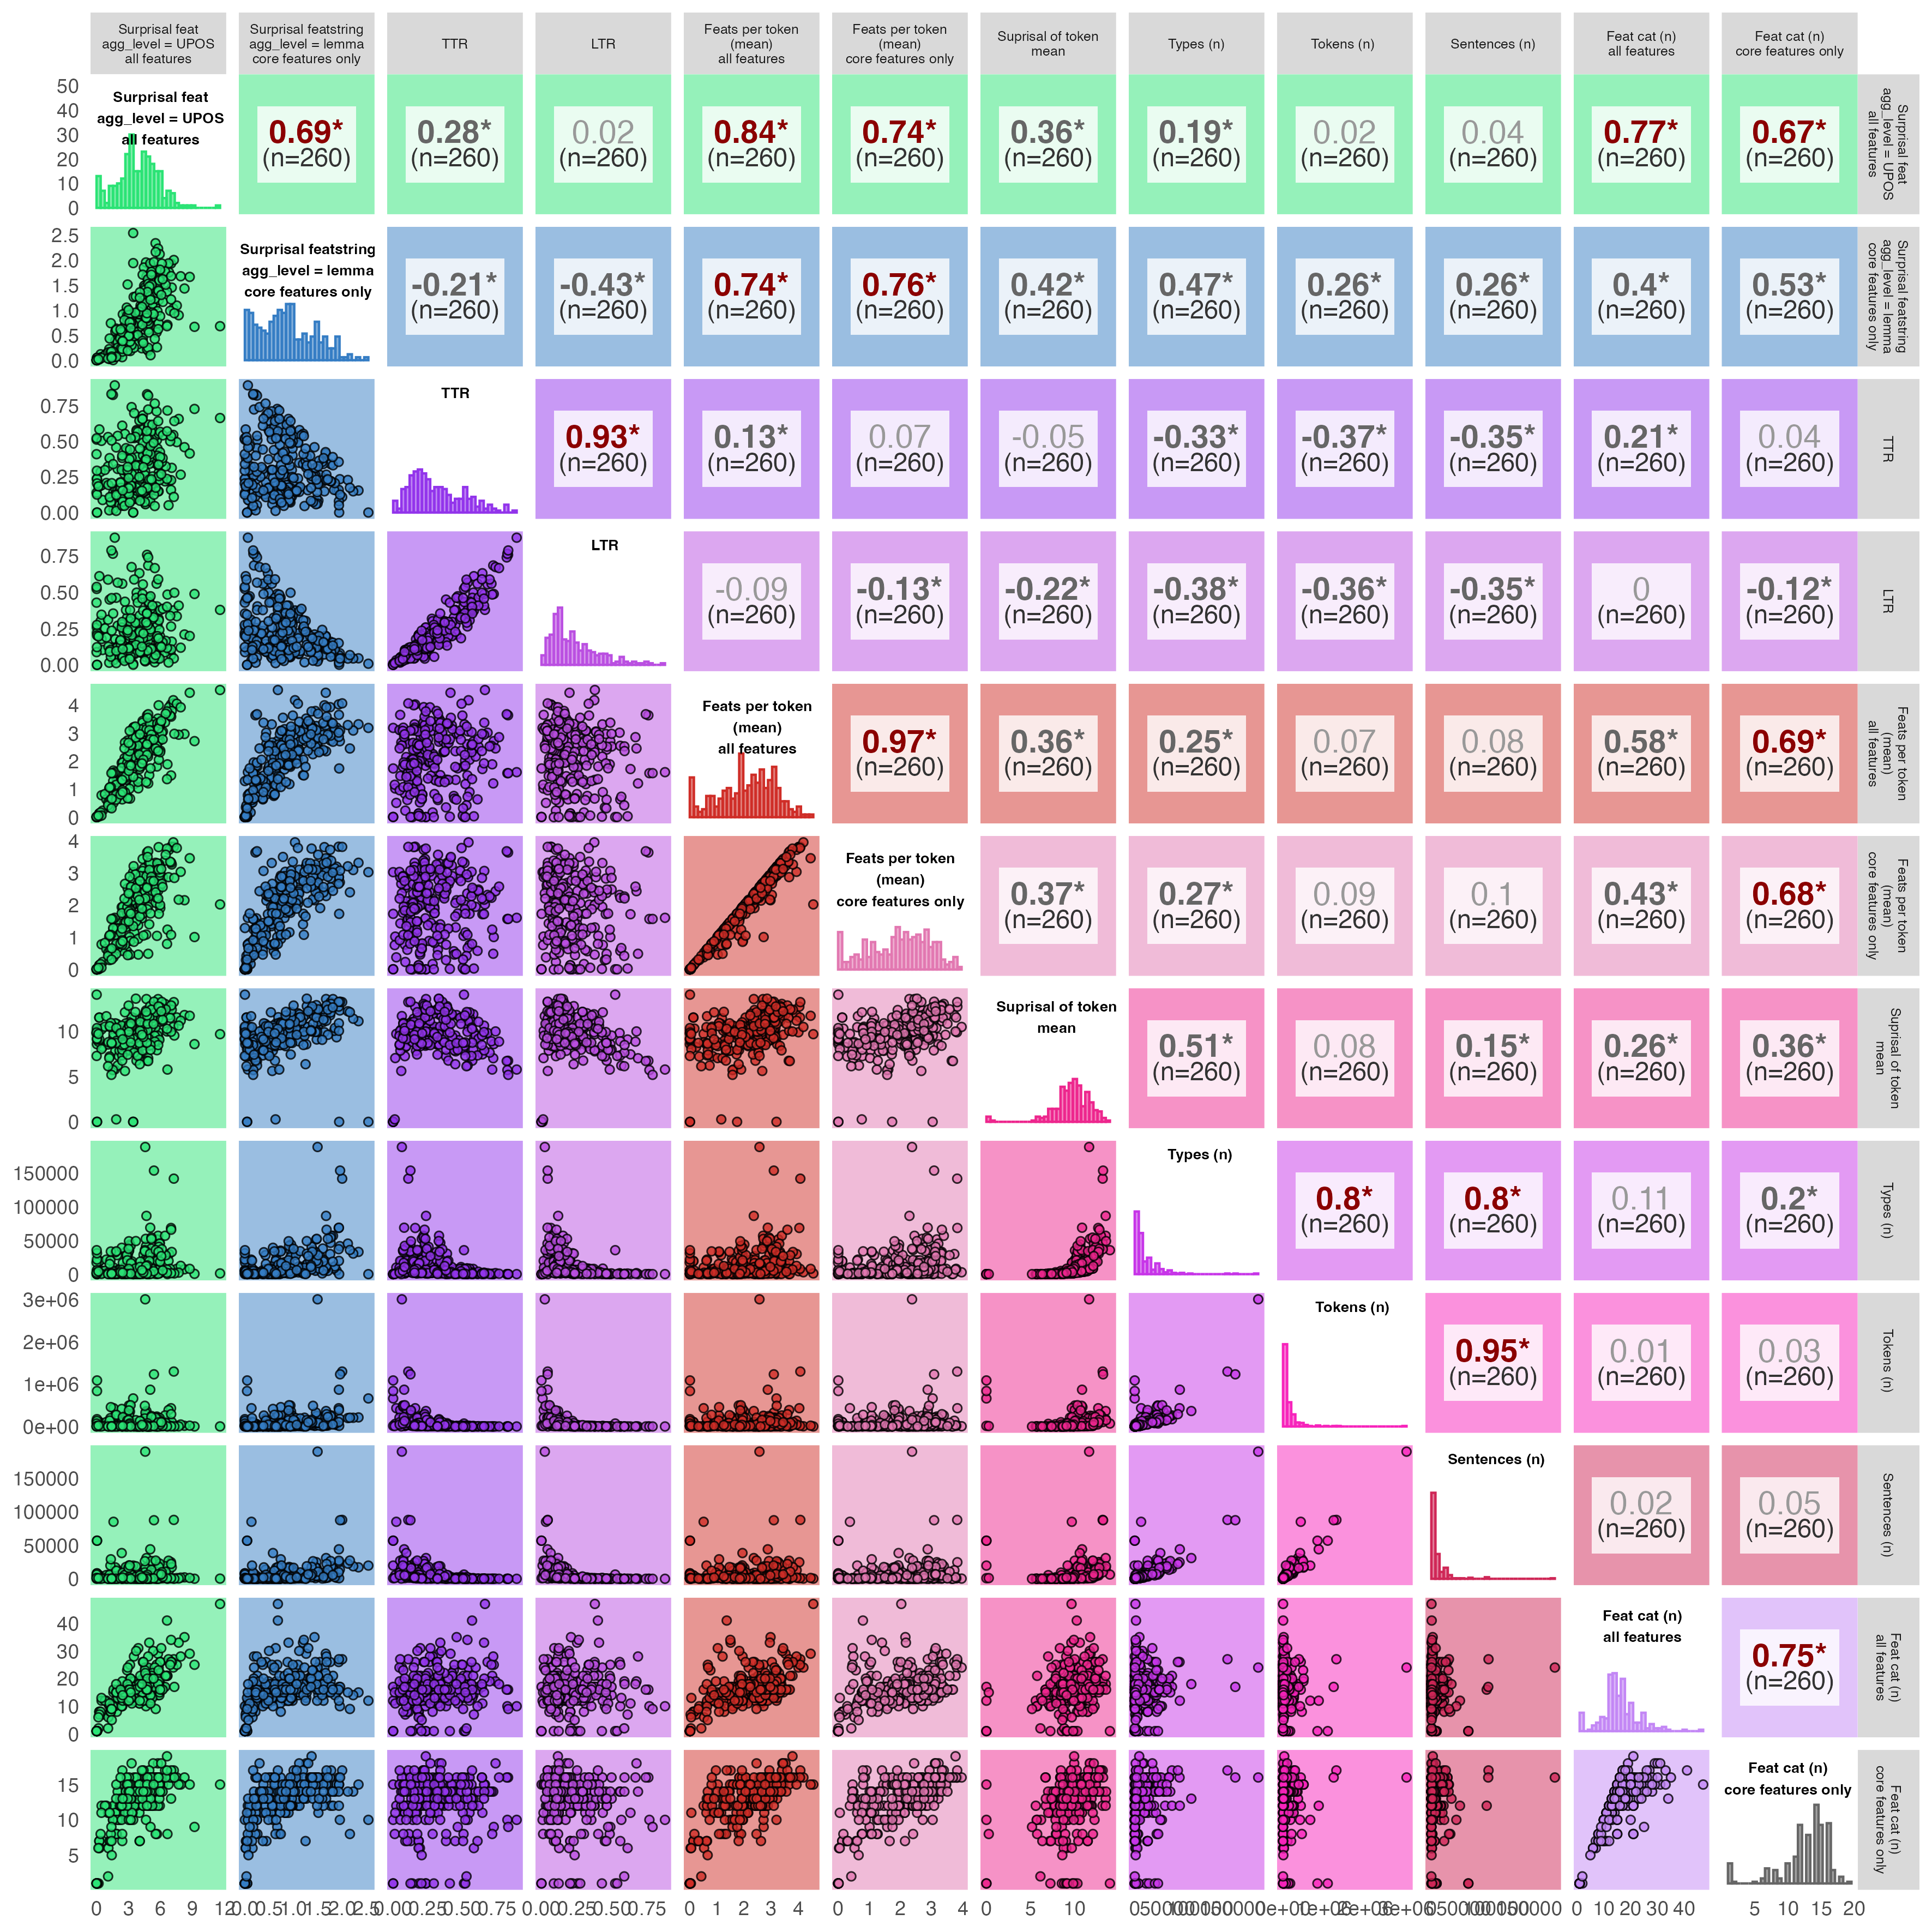
\includegraphics[width=1\linewidth]{latex/graphics/SPLOM_other_metrics.png}
    \caption{SPLOM additional metrics  (all UD datasets). The first two measures are representatives of our custom measures shown in Figure \ref{fig:SPLOM_custom_metrics}, while the remaining measures are standard quantities calculated from the UD datasets.}
    \label{fig:SPLOM_other_metrics}
\end{figure}

\begin{figure}
    \centering
        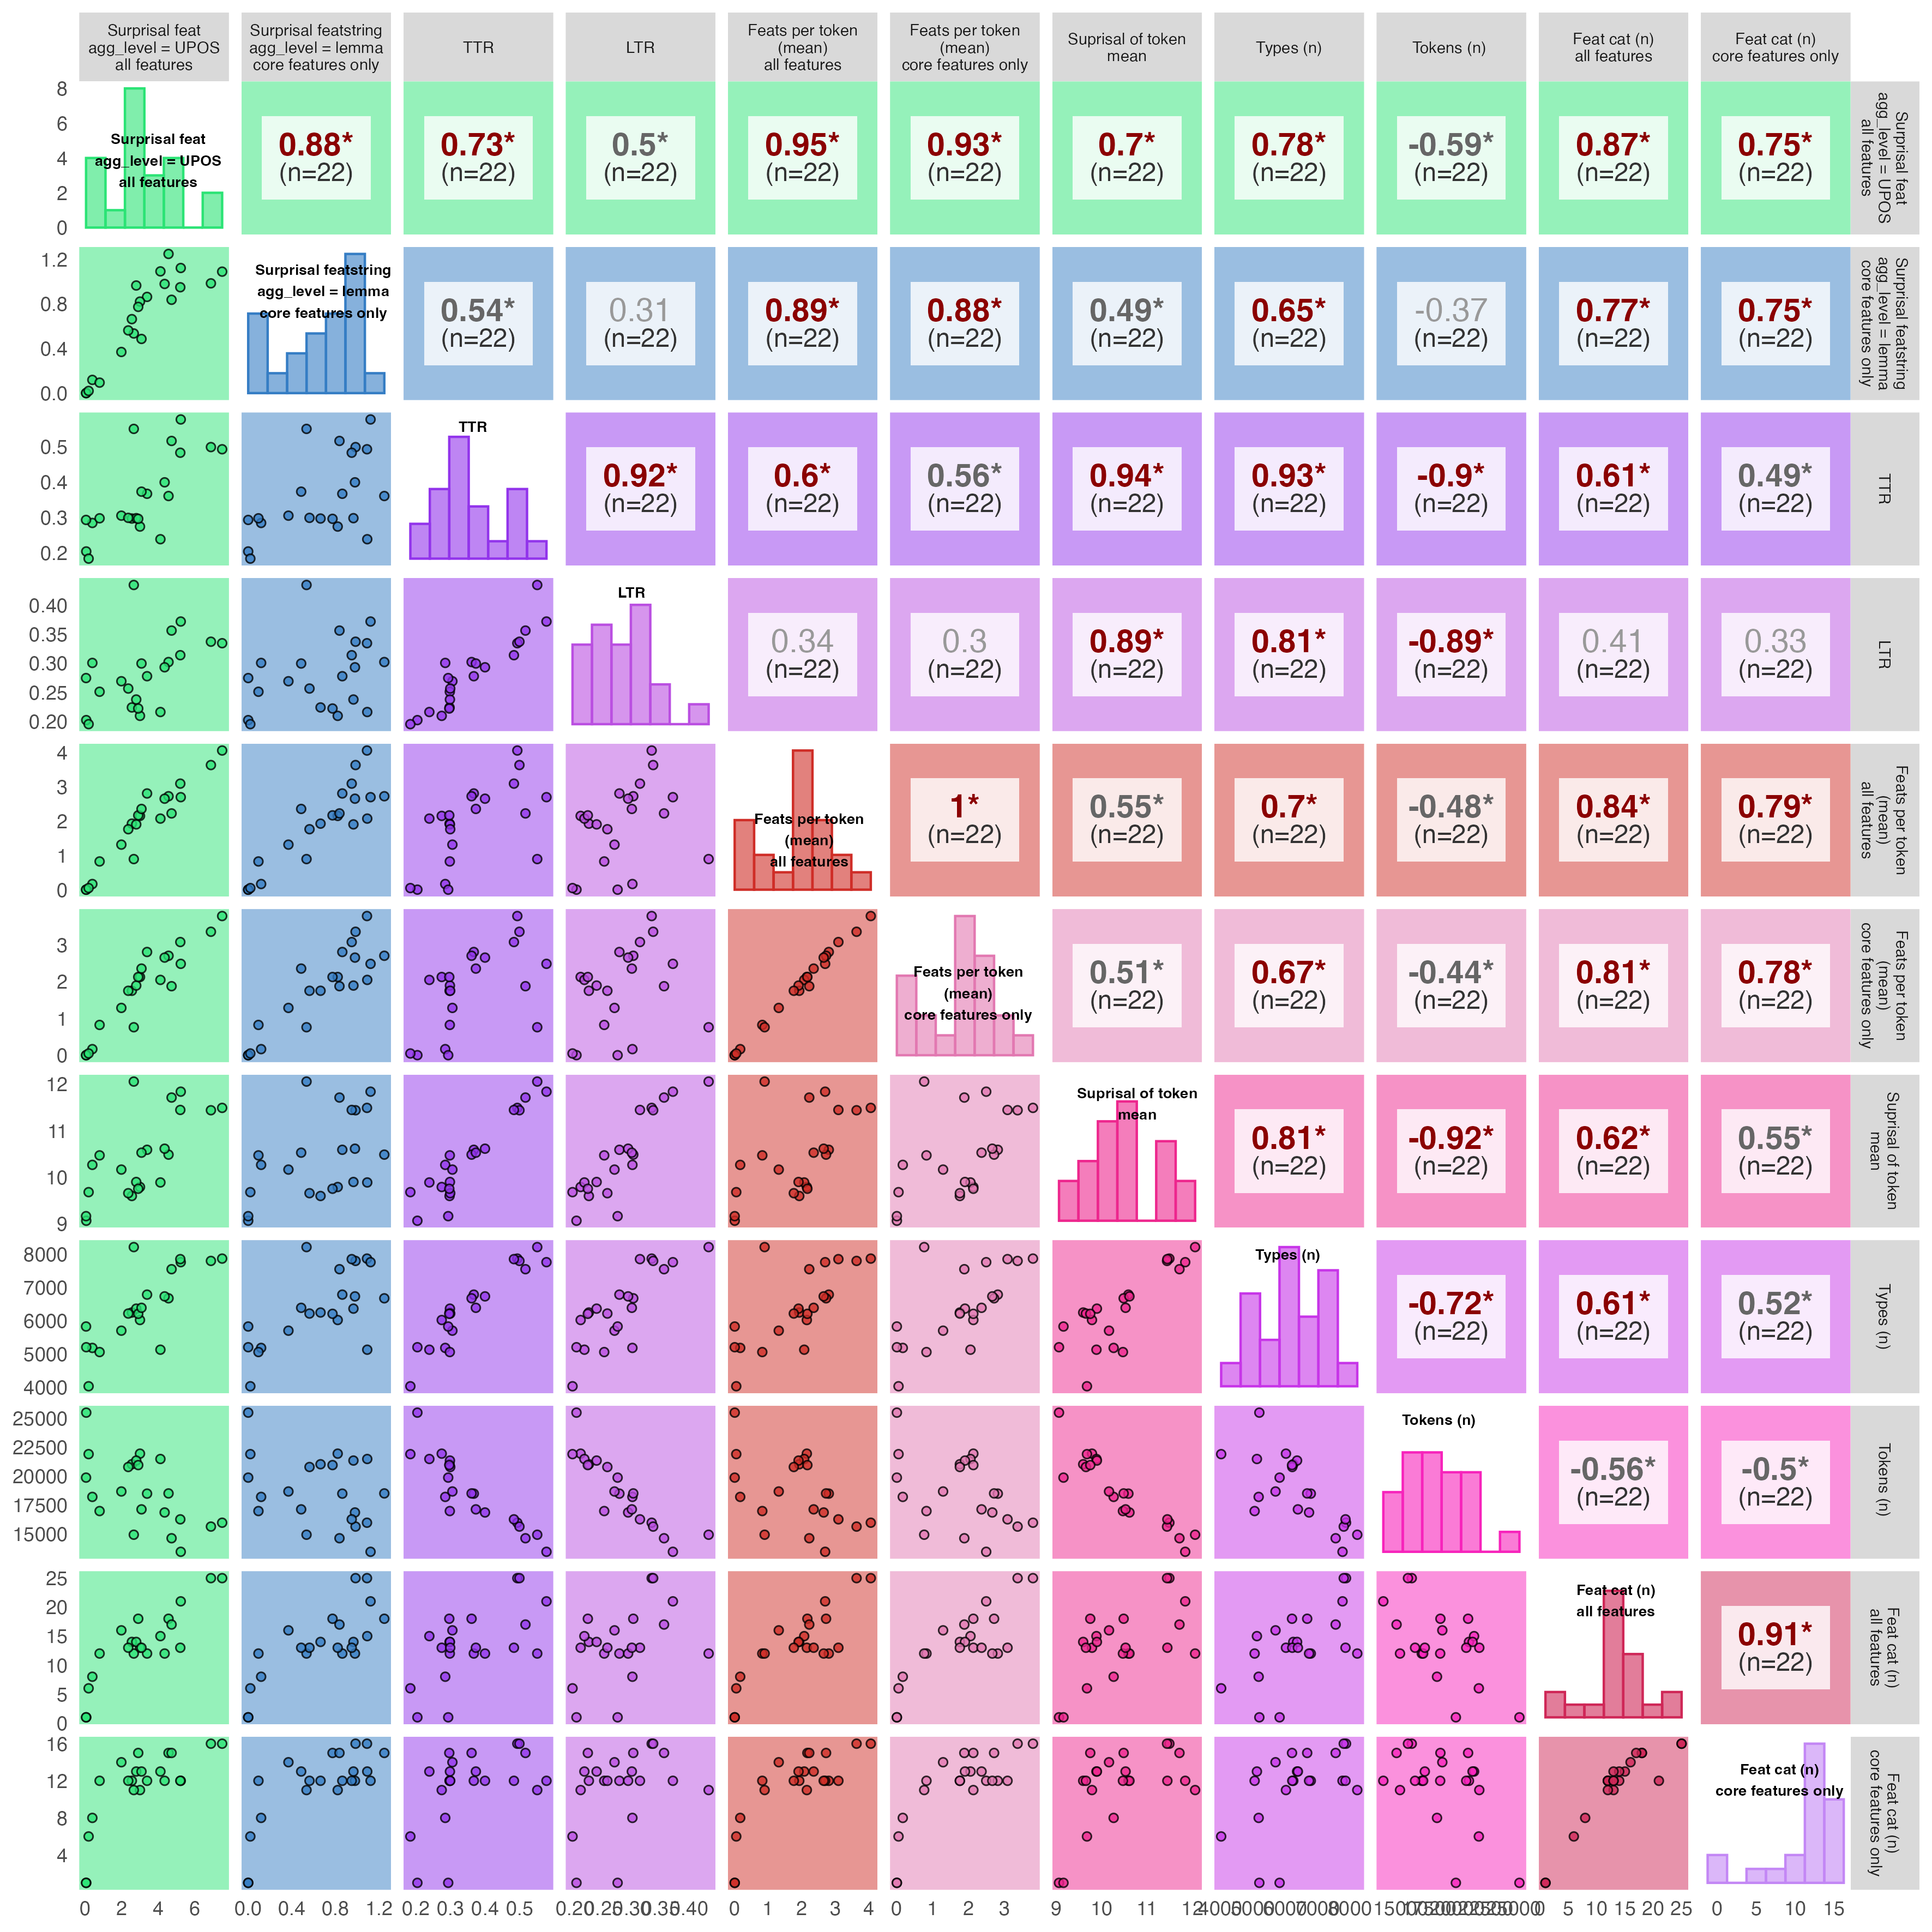
\includegraphics[width=1\linewidth]{latex/graphics/SPLOM_other_metrics_PUD.png}
    \caption{SPLOM additional metrics (PUD datasets only). The first two measures are representatives of our custom measures shown in Figure \ref{fig:SPLOM_custom_metrics_PUD}, while the remaining measures are standard quantities calculated from the PUD datasets. Number of sentences is not displayed as it is fixed for all PUD datasets (1,000 sentences).}
    \label{fig:SPLOM_other_metrics_PUD}
\end{figure}

\subsection{Grambank metrics and population size}
Third, the correlations between our metrics and those calculated from Grambank data are typically weak (Figures \ref{fig:SPLOM_metrics_external} and \ref{fig:SPLOM_metrics_external_PUD}).
Only with the PUD datasets do we see strong correlations, between our two representative metrics and the Grambank Fusion measure, though these are generated by a relatively small sample of only 18 datasets.
This relative dearth of correlations highlights the importance of corpus-based analyses of complexity: insofar as our range of metrics captures something real, it is something that shows up in feature frequencies characteristic of actual language use, rather than the rules describing a language's grammar.
The facets of language complexity discussed earlier (and shown in Figure \ref{fig:metrics_diagram}) are sensitive not just to grammar but to usage, indicating the relevance of corpora for quantifying complexity.
We discuss these issues in more detail below.

Finally, we see weak, though significant, negative correlations between our UPOS-level metric and Google's population measures (both original and log-transformed).
This correlation becomes weaker when we consider our lemma-level metric together with population, and disappears entirely when we also log-transform the population count.

\begin{figure}
    \centering
        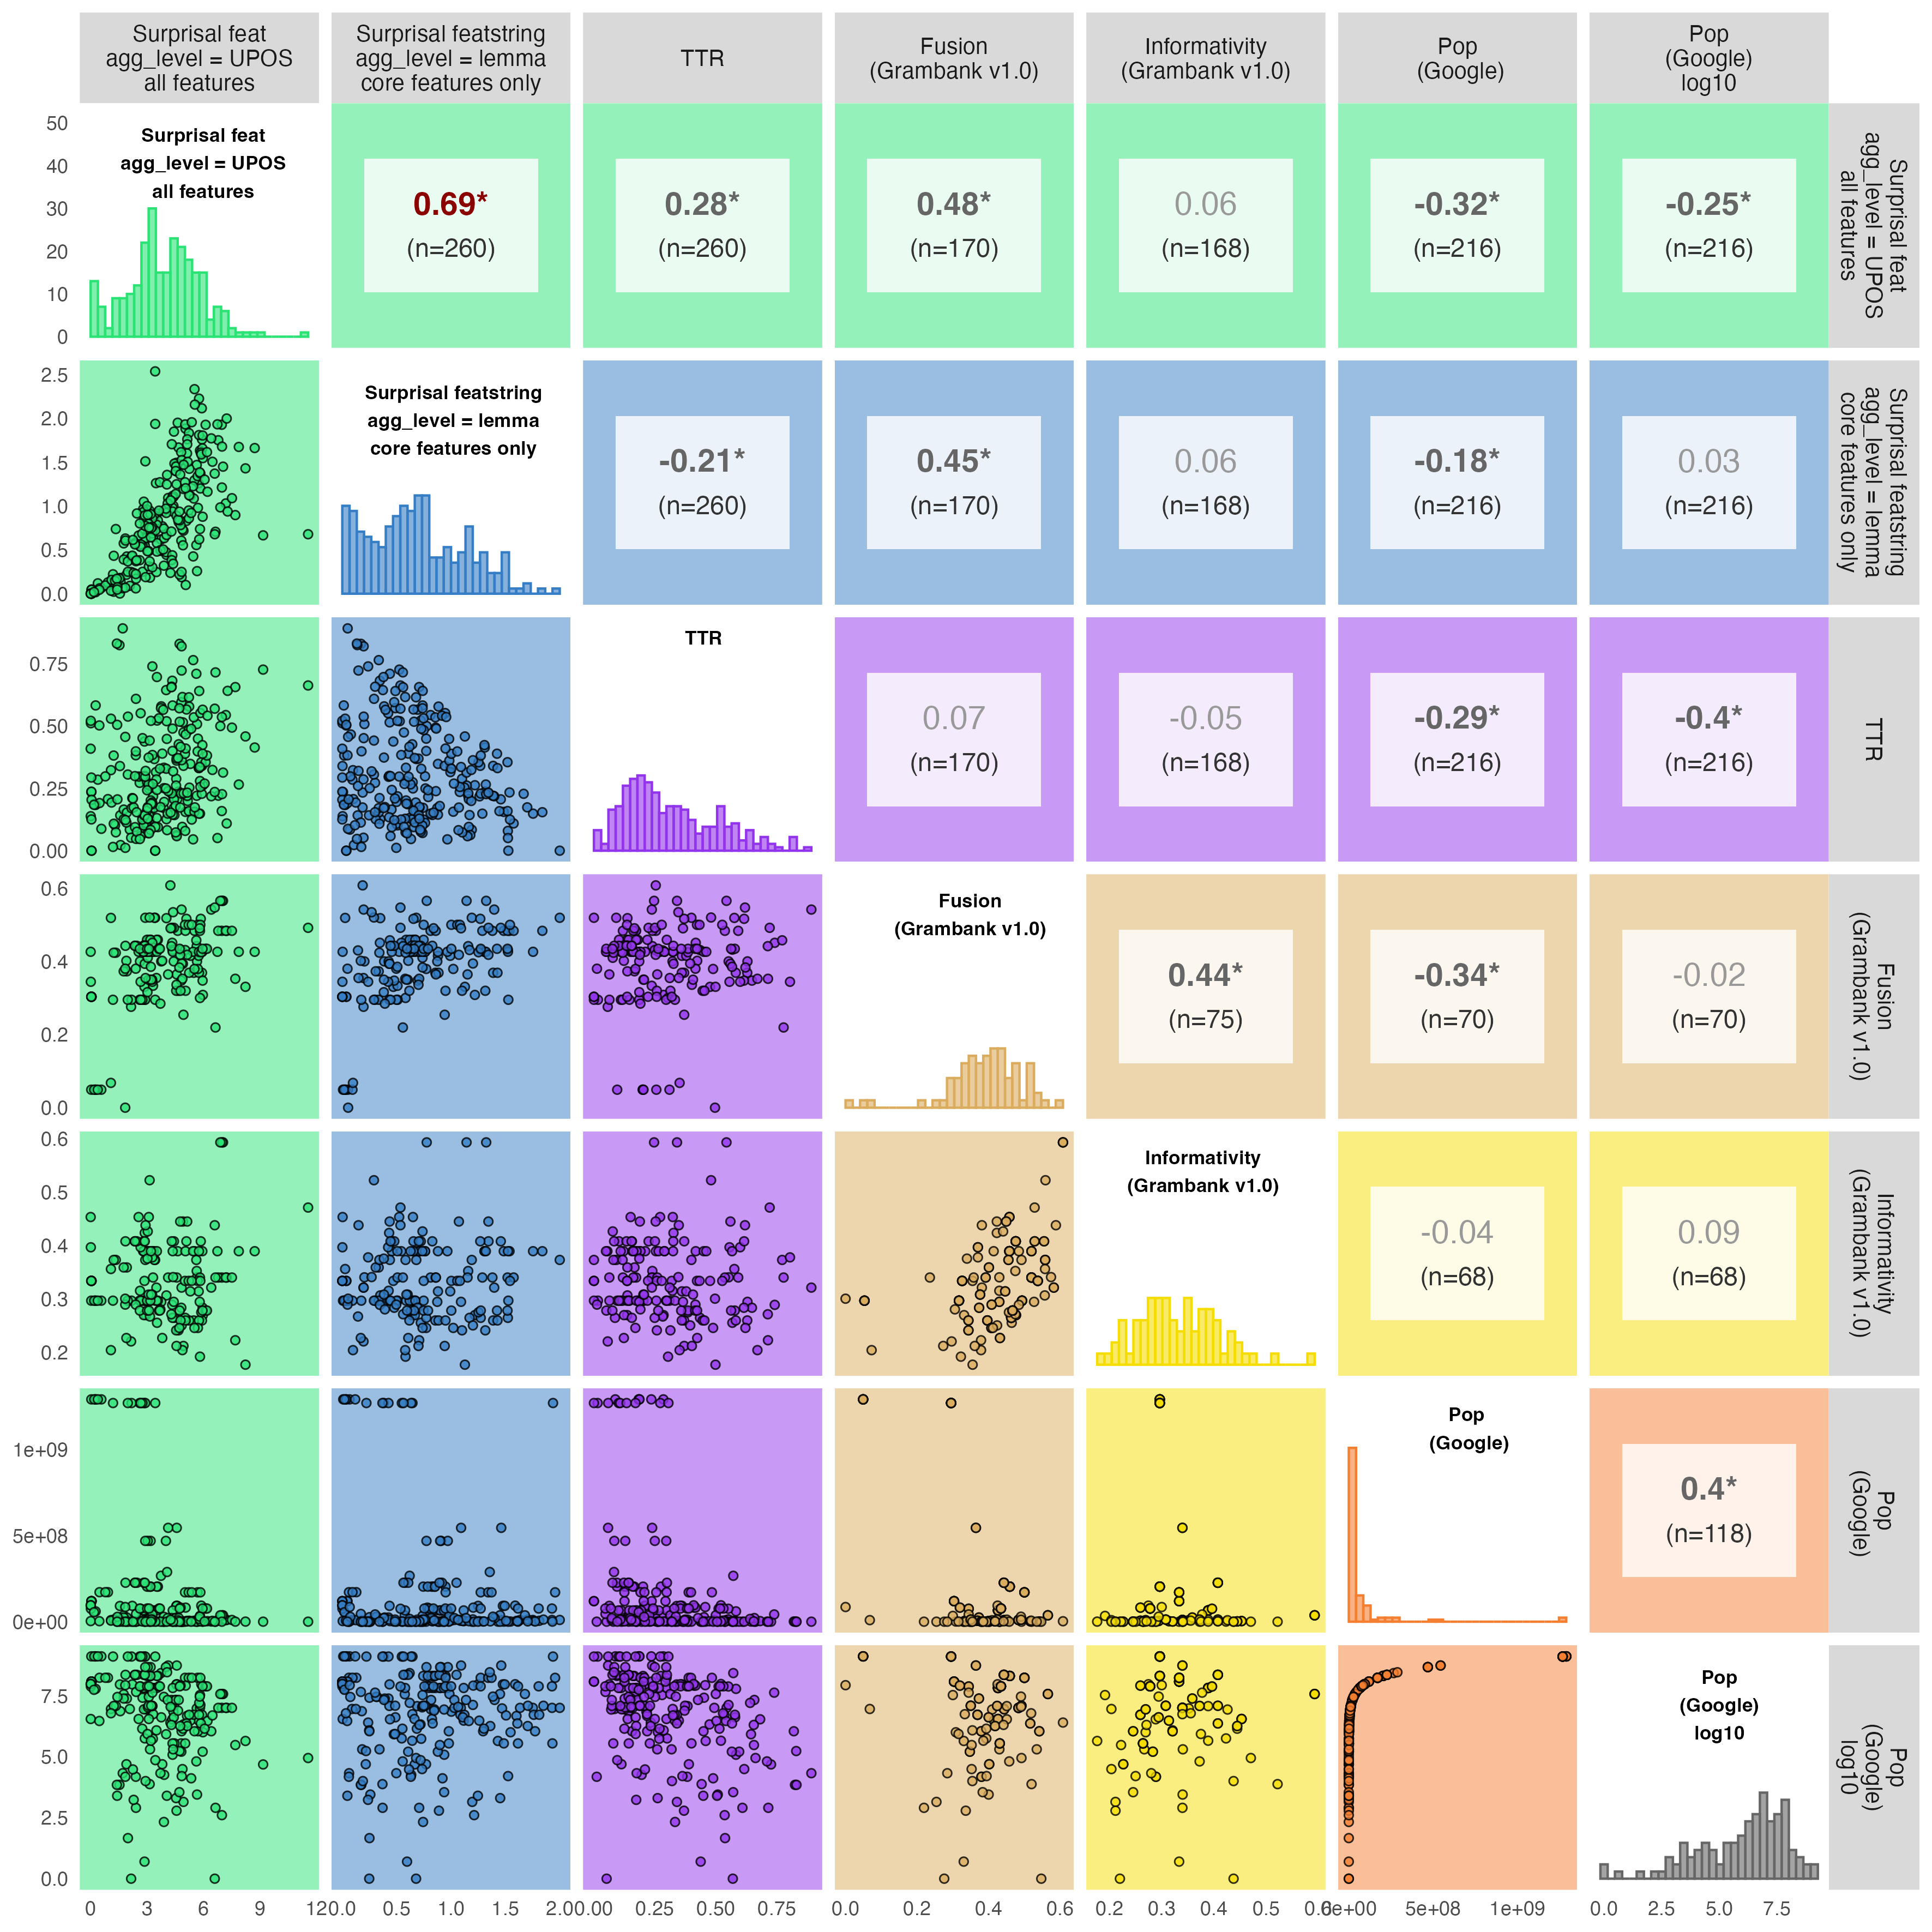
\includegraphics[width=1\linewidth]{latex/graphics/SPLOM_metrics_external.png}
    \caption{SPLOM representative custom metrics, type-token ratio (TTR), Grambank metrics and Google population information  (all UD datasets).}
    \label{fig:SPLOM_metrics_external}
\end{figure}

\begin{figure}
    \centering
        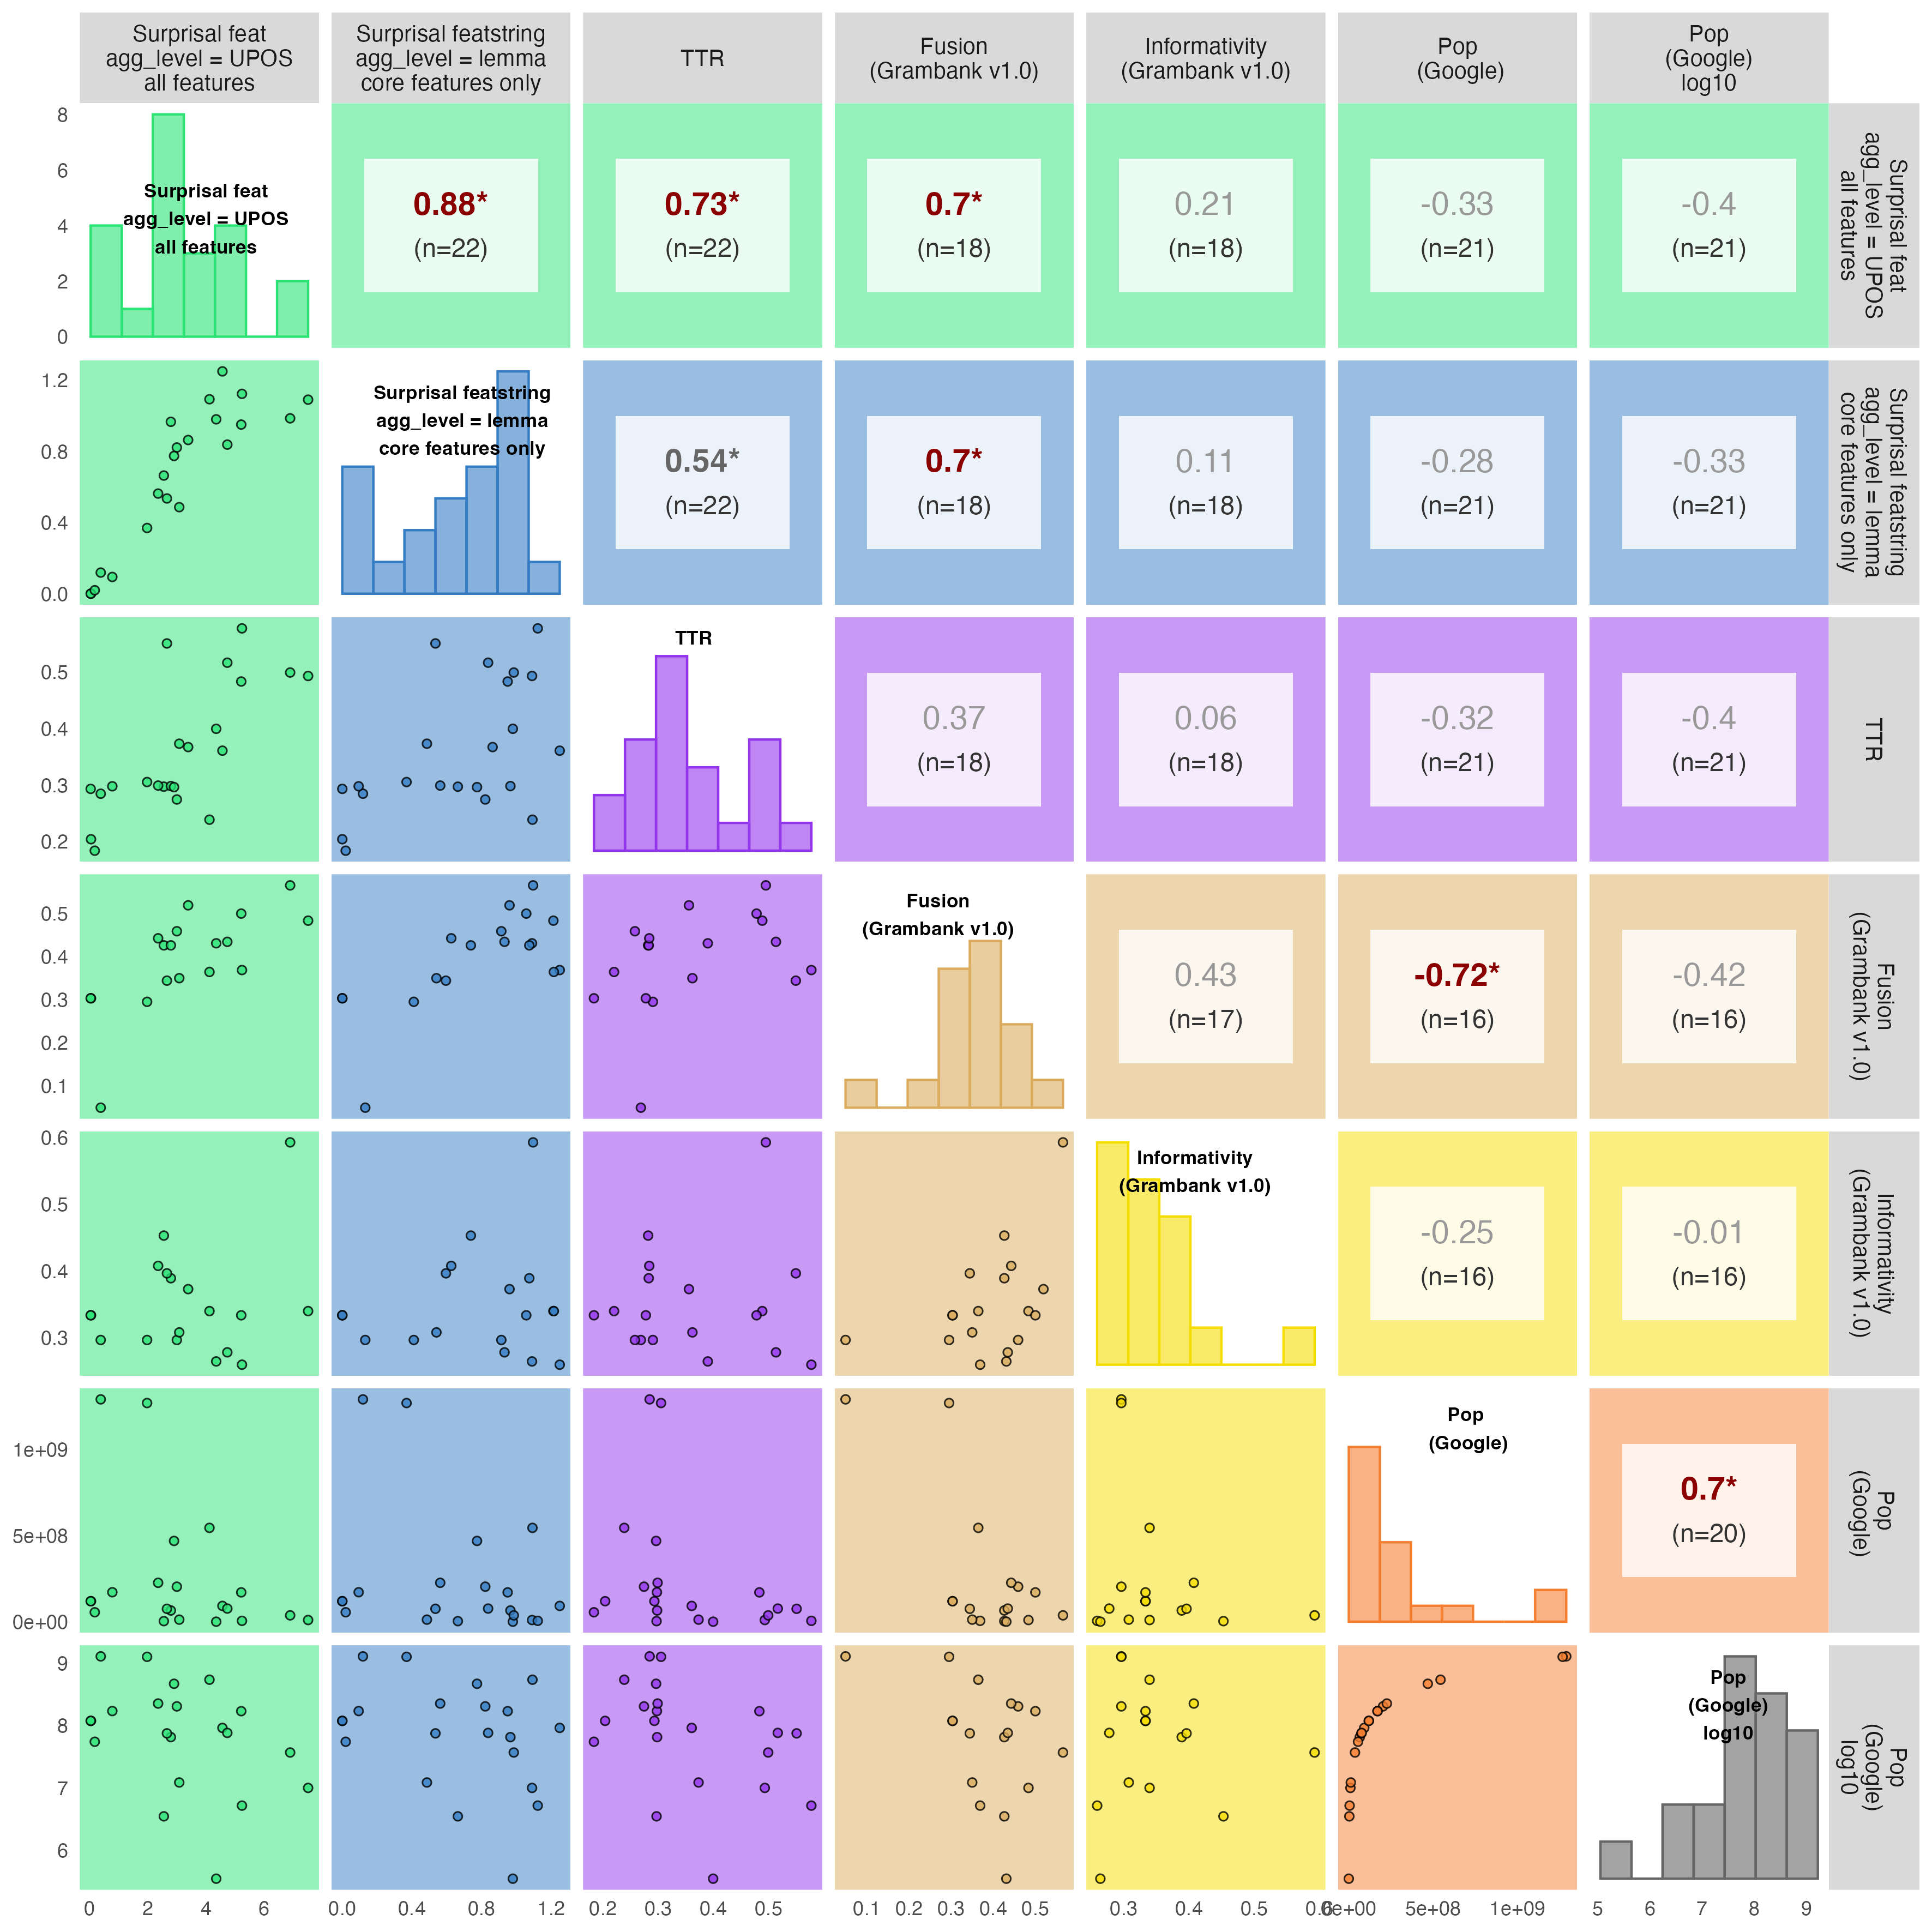
\includegraphics[width=1\linewidth]{latex/graphics/SPLOM_metrics_external_PUD.png}
    \caption{SPLOM representative custom metrics, type-token ratio (TTR), Grambank metrics and Google population information  (PUD datasets only).}
    \label{fig:SPLOM_metrics_external_PUD}
\end{figure}

\FloatBarrier
\section{Discussion}
Overall, the different metrics we define in this paper tell a similar story. 
They all strongly correlate with each other ($>=0.72^*$, see Figures  \ref{fig:SPLOM_custom_metrics} and \ref{fig:SPLOM_custom_metrics_PUD}). 
The difference between the full data and the PUD subset (Figures  \ref{fig:SPLOM_other_metrics} and \ref{fig:SPLOM_other_metrics_PUD}) suggests that genre has a considerable impact on the variation of types in the datasets. 
Corpus-based analyses should therefore take genre into account, and even statistically control for it where possible.

The two custom metrics used for broader comparison in this study correlate either moderately ($0.45^*-0.48^*$) or strongly ($0.7^*$) with the Fusion metric derived from the Grambank dataset \citep{grambank_release, shcherbakova2023societies}, see Figures \ref{fig:SPLOM_metrics_external} and \ref{fig:SPLOM_metrics_external_PUD}. 
This suggests that they are capturing related phenomena. 
Our metrics and Fusion are also connected to the mean number of features per token: the more features in a dataset, the more scope each token has to increase its surprisal; likewise, having more features annotated in a corpus strongly increases a language's chance of being awarded a higher Fusion score based on a grammatical description of the same language.
We do not find the same pattern when comparing our custom metric to the Grambank Informativity metric. 
This may be due to differences in design choices of which grammatical domains to include in the two datasets (UD versus Grambank).
% This relationship can also be seen in the strong correlations between our custom metrics and the mean number of features per token. 
% The more morphological features a language has, the higher the Grambank Fusion score is and the more  

The comparisons of the custom metrics, additional metrics and Grambank metrics is interesting as it shows us that while they differ conceptually, for many pairs the difference is not large. 
The correlations with established metrics (TTR, Fusion etc.) also assures us that we are not entirely off the mark. 
Even though the approaches differ we would expect them to at least weakly correlate - which most of them do. 
However, this should not be taken to mean that it is irrelevant which metric of morphological information/complexity we choose. %(or combination of metrics, see \cite{ccoltekin2023complexity})'s dimensionality reduction proposal)
Which metric is most appropriate should be decided \textit{a priori} based on the conceptual underpinnings and theoretical support it has generally, and by reference to the specific research question.
As we are interested in the informational load of grammar and how language communities make use of it, the custom metrics defined in this paper align more with this aim than the other metrics discussed. 

The results show a weak negative correlation between most of the configurations of the two representative custom metrics and population size (see Figure \ref{fig:SPLOM_metrics_external}). 
This trend is not significant for the PUD dataset, which might be due to the smaller sample size (n=21) or the fact that controlling for genre distorts the relationship.
A negative correlation is in keeping with theoretical expectations as laid out in section \ref{sec:background}. 
%Larger populations increase the probability of interacting with someone with whom you share little common ground, which in turn engenders a greater 
%Less shared common ground > more low-context communication > more information in linguistic code > more information in grammar.
However, it is necessary to investigate this with more sophisticated analyses than a Pearson correlation test.
For example, it is desirable to increase the sample size of comparable corpora and introduce controls for phylogenetic and spatial covariance \citep{shcherbakova2023societies}.

\section{Conclusion}
This paper had three aims:

\begin{enumerate}
    \item Develop a corpus-based metric of morphological information, as a proxy for one aspect of linguistic complexity
    \item Improve on existing measures by explicitly quantifying absent morphological features
    \item Provide a platform for future investigation into pragmatic constraints on grammar
\end{enumerate}

We find it is possible to utilise cross-linguistic corpora such as the UD datasets to explore morphological information in a sophisticated way with information-theoretic approaches. 
Our approach improves upon previous studies such as \citet{ccoltekin2023complexity} by taking into account tokens without morphological features when calculating the overall statistic for the entire dataset and stratifying surprisal by categories (UPOS or lemma). 
To address concerns of non-comparability due to design choices of specific UD dataset contributors, we compute our metrics both over all features annotated and only the core features which are centrally defined by the UD coordinators. 
To caution against non-comparability due to genre, we also present the results for all UD datasets and only those found in the PUD data. 
We find that our corpus-based measures of surprisal typically correlate weakly or not at all with grammar-based measures of Fusion and Informativity (with stronger correlations on a restricted subset), signifying that the aspects of language complexity relating to morphological information are revealed in higher resolution when looking at actual corpora.
Although grammar specifies possibilities and prohibitions, it is usage patterns that primarily determine the difficulty of language learning, production, and comprehension.
% See appendix \ref{sec:caveat_genres} for more discussion of caveats.

% The availability of datasets such as UD \cite{UD_2.14}

%TC:ignore

\bibliographystyle{unified}
\bibliography{bib.bib, used_pkgs}

%\section{Acknowledgements}
%We are indebted to Matthew Spike for his input on this article in particular and for our discussions on ``complexity'' and information in general. We thank {\c{C}}a{\u{g}}r{\i} {\c{C}}{\"o}ltekin and Taraka Rama for their aid in understanding the intracies of their measurement. We also want to thank the audiences at the Working Group for Empirical Linguistics-seminar series (WoGEL) at the Department of Linguistics and Philology at Uppsala University, department seminars at the Department of Linguistic and Cultural Evolution (DLCE) at the Max Planck Institute for Evolutionary Anthropology and participants at the 2024 Biennial meeting of the Association for Linguistic Typology in Singapore. We have also benefitted from advice from Daan van Esch, code review by Christoph Rzymski and discussions with Angela Chira. Finally, we'd like to thank the organisers of the workshop on Dependency Grammar for Typology at the ALT-meeting and editors of this special issue: Andrew Dyer, Luigi Talamo, Annemarie Verkerk, Luca Brigada Villa, Erica Biagetti \& Diego Alves. 

%Luigi, on behalf of Erica, Diego & Luca

\newpage


\setcounter{section}{0}
\renewcommand\thesection{\Alph{section}}
\section*{Appendices}

\section{Detailed procedures}

\subsection{Çöltekin \& Rama}\label{sec:appendix_ccoltekin}

Like us, Çöltekin \& Rama aim to capture how evenly spread are the morphological features of a language.
The canonical mathematical way to measure this `even-spreadedness' is entropy.
Defined as $\Sigma p \log{\frac{1}{p}}$ for probabilities $p$ of a given distribution, entropy is large when probabilities are more evenly distributed and small when a few probabilities are much greater than the others.
Thus entropy captures something like the average amount of uncertainty among a set of items.
Çöltekin \& Rama thus define a measure of the entropy of all morphological features in a dataset to capture one aspect of a language's complexity.
Their method of calculating this value is as follows:\footnote{This procedure describes the code which can be found at \url{https://github.com/coltekin/mcomplexity/blob/main/mlc-morph.py}, specifically the method \texttt{get\_mfh}.} %We are grateful to Çöltekin \& Rama for corresponding with us so that we could confirm our understanding of their procedure. Any remaining misunderstandings are our own.}:
\begin{enumerate}
\item For a given dataset, randomly sample a fixed number of tokens
\item Remove punctuation (UPOS=`PUNCT') and unanalysable tokens (UPOS=`X')
\item Remove tokens that have no morphological features
\item Split the remaining tokens' morphological features into a list (e.g. Table \ref{tab:mfh} lists the individual features in the sample shown in Table \ref{tab:turkish_example})
\item Count how many times each feature occurs in the sample (column `Count' in Table \ref{tab:mfh})
\item Calculate the relative frequency of each feature (column `Frequency (p)' in Table \ref{tab:mfh}; this is the feature's Count value divided by the sum of the Count column for the entire sample)
\item Calculate entropy from the frequencies ($\Sigma p \log{\frac{1}{p}}$)
\item Run steps 2-7 multiple times for different samples of the same size and take the mean entropy.
\end{enumerate}

\noindent Table \ref{tab:mfh} shows the components of the entropy measure for the sample of tokens listed in Table \ref{tab:turkish_example}.
The total entropy for this sample is approximately 3.15 bits.
In their study \citet{ccoltekin2023complexity} would sample something like 1000 tokens at a time, generating an entropy measure each time and then taking the average.
This average is then an estimate of the `overall' entropy measure for the dataset.

\begin{table}[h]
    \centering
    \caption{Components of the measure of morphological feature entropy as defined by \citet{ccoltekin2023complexity} for the sample of tokens in Table \ref{tab:turkish_example}. The total feature count is 17, and each feature's Frequency is its Count divided by this total (rounded to three significant figures). The entropy of this sample is 3.15 bits (also to three significant figures).} %note table captions go above the table
    \label{tab:mfh}   
    \begin{tabular}{p{5cm}p{3cm}p{3cm}}
\toprule
	\textbf{Morphological feature}	&	\textbf{Count}	&	\textbf{Frequency (p)}	\\
    \midrule
	Case=Loc&1&0.0588       \\    \midrule
	Number=Sing&4&0.235    \\    \midrule
        Person=3&4&0.235		   \\    \midrule
	Case=Nom&1&0.0588	       \\    \midrule
	Case=Acc&1&0.0588		      \\    \midrule
        Aspect=Perf&1&0.0588      \\    \midrule
        Mood=Ind&1&0.0588		   \\    \midrule
        Polarity=Pos&1&0.0588		\\    \midrule
	Tense=Past&1&0.0588	     \\    \midrule
	VerbForm=Fin&1&0.0588	    \\    \midrule
	Voice=Cau&1&0.0588      	\\ \bottomrule

    \end{tabular}
\end{table}

\subsection{The present study}\label{sec:appendix_ours}

\subsubsection{Procedure for measuring mean surprisal per token}

The full procedure of our basic metric is as follows:
\begin{enumerate}
\item Combine the files of each UD dataset (e.g. dev, test and train) to one table with one token per row
\item Remove punctuation (UPOS=`PUNCT'), symbols (UPOS=`SYM') and unanalysable tokens (UPOS=`X')
\item Define lemmas as a combination of lemma + UPOS, so that lemmas that are spelled the same but belong to different UPOS can be distinguished. \textit{Example:} the noun ``mark'' and the verb ``mark'' in English are defined as having the lemmas ``mark\_NOUN'' and ``mark\_VERB'' as opposed to both potentially being assigned to the same lemma ``mark''.
\item Determine the full set of morphological feature categories per lemma. \textit{Example:} the token `sebuah' in Table \ref{tab:unassigned_ex} has features Definite and PronType; supposing there were another token of the same lemma in the dataset that had a value for the category Number, then the full set of categories for `sebuah' would be Definite, Number and PronType.
\item Remove features that are not related to morphology: ``Abbr'' (abbreviations), ``Typo'' (whether or not a token has a typo) and ``Foreign'' (whether or not a token is deemed as in a foreign language)
\item Assign a dummy value to unassigned morphological categories for each token, given the other available feature categories for tokens of the same lemma. \textit{Example:} for `sebuah' we insert the dummy feature Number=unassigned.
\item Split the tokens' morphological features into a list (e.g. Table \ref{tab:unassigned_ex_SPLIT} lists the individual features for the sample shown in Table \ref{tab:unassigned_ex})\footnote{Some tokens have been given more than one feature value for the same feature category. This is allowable within the UD-framework, though the coordinators note that such multi-values should be used sparingly. For example, the adjective ``{\dolousfont ἀ}{\Timesfont όρατος}'' in the Ancient Greek PTNK-dataset is assigned ``Gender=Fem,Masc''. We are treating instances like these as a case of the feature value being ``Fem,Masc'' and not a case of both ``Gender=Fem'' and ``Gender=Masc''.}
\item Count how many times each feature \textit{value} occurs \textit{for that category, in tokens of that lemma} (column `Count' in Table \ref{tab:unassigned_ex_SPLIT})
\item Calculate the relative frequency of each feature value (column `Frequency' in Table \ref{tab:unassigned_ex_SPLIT}; this is the feature value's Count divided by the number of times that lemma appears in the dataset)
\item Calculate the surprisal of that feature value for that token: $\log{\frac{1}{\text{frequency}}}$
\item Calculate the total `surprisal of a token' by summing the surprisals of all its features (including dummy-assigned features)
\item Mean surprisal per token is the average of this total across all tokens in the dataset.

% \item Calculate the mean surprisal in the dataset by summing the surprisals and dividing by the number of tokens.
\end{enumerate}

Clearly our mean surprisal measure is capturing something similar to the classical entropy measure used by \citet{ccoltekin2023complexity}, but they are not strictly equivalent.
Entropy weights surprisal by the same probability that defines the surprisal: the two $p$'s in the formula $\Sigma p\log{\frac{1}{p}}$ are the same.
By contrast our measure calculates a sum of surprisals, each of which is defined in terms of the frequencies of its morphological feature values.
Only then do we calculate a mean value by summing across the entire dataset.
The formula describing our measure is therefore $\Sigma_i p_i \left( \Sigma_{j_i} \log{\frac{1}{p_{j_i}}} \right)$ where $i$ ranges across tokens and $j_i$ ranges across feature values of token $i$.

\begin{table}[h]
    \centering
    \caption{Four tokens from the treebank UD\_Indonesian-PUD. The token `sebuah' has no feature value for Number, but in this illustrative example we imagine that other tokens of the same lemma do have this feature. We therefore include it as an unassigned feature; likewise for `para' and the feature Definite. Of the adjectives, neither `baru' nor `terakhir' have a value for the feature NumType; we continue to imagine that there is at least one lemma for each of these tokens that does have a value for this feature, therefore both are given it as an unassigned feature. In fact the token `baru' has no feature values of its own; thus it takes all features possessed by any other token of the lemma `baru' as unassigned.} %note table captions go above the table
    \label{tab:unassigned_ex}   
    \begin{tabular}{p{1cm}p{1.4cm}p{1.5cm}p{3.5cm}p{2.5cm}}
\toprule

% UD\_Indonesian-PUD
%id	&
UPOS&lemma	&token	&feats & unassigned feats	\\ 
\midrule
DET & buah & sebuah 
& Definite=Ind|PronType=Art
& Number
\\\midrule
DET & para	& para	&Number=Plur|PronType=Ind & Definite
\\\midrule
ADJ&baru	&baru&
& Degree \newline
NumType 
\\\midrule
ADJ & akhir	&terakhir&	Degree=Sup& NumType\\\bottomrule
\end{tabular}
\end{table}

% OUR APPROACH, FEATURES SPLIT
\begin{table}[h]
    \centering
    \caption{Four tokens from the treebank UD\_Indonesian-PUD. For illustrative purposes we imagine this dataset contains 20 occurrences of the lemma `buah', 10 of `para', 5 of `baru' and 12 of `akhir'. The Count and Frequency columns, whose values in this table are also illustrative and not real, answer the question: `how often does this lemma have this value for this feature?'. The frequencies are used to calculate the surprisal of a particular token. For example, the surprisal of the token `sebuah' is $\log{\frac{1}{0.3}}+\log{\frac{1}{0.05}}+\log{\frac{1}{0.5}} = 7.06\text{ bits}$ (to three significant figures).} %note table captions go above the table
    \label{tab:unassigned_ex_SPLIT}   
    \begin{tabular}{p{0.7cm}p{1cm}p{1.4cm}p{1.3cm}p{1.5cm}p{1.4cm}p{1.6cm}}
\toprule

%id	&
UPOS&lemma	&token	&feat name & feat value & Count\newline (illustrative) & Frequency\newline (illustrative)	\\ \midrule

DET & buah & sebuah & Definite& Ind & 6 & 0.3\\
DET & buah & sebuah & Number& unassigned & 1 & 0.05\\
DET & buah & sebuah & PronType& Art & 10 & 0.5
\\\midrule
DET & para	& para	&Definite & unassigned & 1 & 0.1\\
DET & para	& para	&Number & Plur & 4 & 0.4\\
DET & para	& para	&PronType & Ind & 6 & 0.6
\\\midrule
ADJ&baru	&baru& Degree&unassigned & 4 & 0.8\\
ADJ&baru	&baru& NumType&unassigned & 1 & 0.2 \\\midrule
ADJ & akhir	&terakhir&	Degree& Sup & 3 & 0.25\\
ADJ & akhir	&terakhir&	NumType & unassigned & 4 & 0.333\\
\bottomrule
\end{tabular}
\end{table}

\subsubsection{Calculation of Grambank metrics}\label{sec:appendix_rgrambank}

The calculation of Fusion and Informativity from raw Grambank data is somewhat involved.
We combine dialects into languages, and if two dialects under the same language have different values for the same feature, we choose one at random. 
We remove languages with more than 25\% missing data across the features used to calculate each metric. 
We do this using the functions from the package rgrambank \citep{R-rgrambank}. 
This data wrangling procedure differs slightly from \citet{grambank_release} and \citet{shcherbakova2023societies}, but the difference is negligible. 
See example scripts accompanying the R-package rgrambank for illustration of procedure and differences.
Unlike \cite{shcherbakova2023societies}, but like \cite{grambank_release} we use the version of the Grambank metric Fusion which awards features that cover bound morphology and other morphology half a Fusion-point.

\FloatBarrier

\section{Caveats}
\label{sec:caveats}

\subsection{Comparability}
\label{caveat_comparability}
In comparative studies, it is desirable to compare like with like. There are several comparability challenges in this study. These are known and expected with datasets like UD \citep{UD_2.14}. We list the ones that are most important to our study here. 

\subsubsection{Variation in morphological annotation}
Datasets can vary in many aspects, one of them being the \textbf{level of analysis of morphology}. 
Some datasets may contain many different morphological features and some very few, despite the underlying languages being similar. 
This is due to the design choices of the contributors of each dataset, and variation of this kind is expected in a project like UD.
Unfortunately, incompatible levels of annotation or annotation schemes makes the datasets less comparable.
We address this by calculating our metrics once for all features specified in a given dataset and once for the ``universal'' morphological features only. 
The UD-documentation guidelines specify a subset of the morphological features as ``universal'' \citep{ud_2_feat_website}. 
The UD-documentation writes that these are described in a standardised manner, with some flexibility. 
However, ``[t]his does not mean that they occur in all languages. It means that they have been attested in more than one language and they are considered linguistically important. UD treebanks may use additional features and values if they are properly documented'' \citep{ud_2_feat_website}. 
This set of morphological features are defined centrally within the UD-project as a whole, as opposed to defined locally for each UD dataset. 
They are:\footnote{For more detailed definitions of morphological features in the UD datasets, see the UD website. We also note that three features originally included in this list -- Abbr (abbreviations), Typo and Foreign -- are excluded from all of our analyses as they do not correspond to aspects of morphological complexity.}
\begin{itemize}
    \item PronType: pronominal type 
    \item NumType: numeral type
    \item Poss: possessive
    \item Reflex: reflexive
    \item ExtPos: external part of speech
    \item Gender: gender
    \item Animacy: animacy
    \item NounClass: noun class
    \item Number: number
    \item Case: case
    \item Definite: definiteness or state
    \item Deixis: relative location encoded in demonstrative
    \item DeixisRef: person to which deixis is relative
    \item Degree: degree of comparison
    \item VerbForm: form of verb or deverbative
    \item Mood: mood 
    \item Tense: tense
    \item Aspect: aspect 
    \item Voice: voice
    \item Evident: evidentiality
    \item Polarity: polarity
    \item Person: person
    \item Polite: politeness
    \item Clusivity: clusivity
\end{itemize}

As core features are more standardised across UD datasets, albeit with some flexibility, we expect these features to be the most comparable across datasets.\footnote{For an example of this flexibility, the UD guidelines note that while gender is commonly associated with nouns, there is nothing in the central guidelines that prevent the feature from also appearing on adjectives and verbs.}
We use the term ``core'' in this paper for this class of morphological features so as to not confuse it with other senses of the term ``universal''.

\subsubsection{Variation in Universal Part-Of-Speech annotation (UPOS)}
The UD datasets use a specific set of Universal Part-Of-Speech categories (UPOS):

\begin{itemize}
    \item ADJ: adjective
    \item ADP: adposition
    \item ADV: adverb
    \item AUX: auxiliary
    \item CCONJ: coordinating conjunction
    \item DET: determiner
    \item INTJ: interjection
    \item NOUN: noun
    \item NUM: numeral
    \item PART: particle
    \item PRON: pronoun
    \item PROPN: proper noun
    \item PUNCT: punctuation
    \item SCONJ: subordinating conjunction
    \item SYM: symbol
    \item VERB: verb
    \item X: other
\end{itemize}

These are defined centrally across datasets, but as with morphological features there is also language specific variation in how they are defined and applied. 
Parts-Of-Speech/word classes famously vary across languages in terms of which ones exist, how they behave, how they subdivide further, and so on. 
Some languages do not have an identifiable class of adjectives, with such meanings instead being expressed with nouns or verbs. 
Some languages have a fluid boundary between nouns and verbs. 
There is a substantial literature in linguistic theory and typology that deals with the definition of parts-of-speech/word classes across languages (c.f. \citet{kira_keira}).
For this project, we are naturally dependent on how the UD-central team have defined these labels and how the contributors of each dataset have then further specified them.

For example, in the UD dataset Abaza-ATB (glottocode = abaz1241, ISO 639-3 abq) there are tokens which are marked as having UPOS VERB but which have very different morphological features. 
Consider the token {\Timesfont цIитI} in Table \ref{tab:Abaza_sent_10} and {\Timesfont йазкIкIыта} in Table \ref{tab:Abaza_sent_11} which are both marked as UPOS VERB. 
The first token, {\Timesfont цIитI}, is annotated for features often associated with finite verbs such as tense. 
The token {\Timesfont йазкIкIыта} is likewise also tagged as UPOS VERB, but the morphological features are quite different. 
The morphological features of {\Timesfont йазкIкIыта} are all related to the gender, person and number of the arguments of the verb (io = indirect object, abs = absolutive). 
The two tokens do not share any features: {\Timesfont цIитI} is not marked for gender/person/number of the arguments and {\Timesfont йазкIкIыта} is not marked for tense or VerbForm.
Based on studying these annotations alone, we may reach the conclusion that there are at least two categories of tokens which are both included under the heading VERB and that have very different morphological behaviour.
This is not unexpected and is likely to occur for many datasets in UD, to different degrees.

\begin{table}[]
    \centering
    \begin{tabular}{p{3cm}|p{8cm}}
    Abaza     & {\Timesfont{щарда \underline{цIитI} ари агIаншижьтара}} \\
    Russian    & {\Timesfont{С тех пор прошло много времени }}\\
    English & A lot of time has passed since then\\
    Morphological features & Tense=Pres|VerbForm=Fin \\
    \end{tabular}
    \caption{Sentence 10 from UD dataset Abaza-ATB (UD v2.14). Only the morphological features for the underlined word are listed.}
    \label{tab:Abaza_sent_10}
\end{table}

\begin{table}[]
    \centering
    \begin{tabular}{p{3cm}|p{8cm}}
    Abaza     & {\Timesfont{апхъа азаман уагIахъата адунай йыквыз шабгаз \underline{йазкIкIыта} зджьара йбзазун }}\\
    Russian    &{\Timesfont{В то время люди, которые находились на свете, собравшись, жили где-то }}\\
    English & At that time, the people who were in the world, having gathered, lived somewhere\\
    Morphological features & Gender[io]=Neut|Number[abs]=Plur|Number[io]=Sing| Person[abs]=3|Person[io]=3 \\
    \end{tabular}
    \caption{Sentence 11 from UD dataset Abaza-ATB (UD v2.14). Only the morphological features for the underlined word are listed.}
    \label{tab:Abaza_sent_11}
\end{table}

The UD annotation guidelines states that a verb ``is a member of the syntactic class of words that typically signal events and actions, can constitute a minimal predicate in a clause, and govern the number and types of other constituents which may occur in the clause'' \citep{ud_2_VERB_website}. 
They go on to note that the UPOS-label VERB is not applied to auxiliary verbs. 
The documentation further specifies that, depending on language-specific analysis, (i) participles may be tagged as VERB or ADJ, (ii) gerunds and infinitives may be analysed as VERB or NOUN and that (iii) converbs (transgressives) or adverbial participles may be classed as VERB or ADV.
This standardised definition therefore still leaves a lot of flexibility, as is desirable and expected in a project of this kind.

Given the structure of the language at hand and the specific decisions of the contributors, this can mean that the Parts-Of-Speech-topology can differ a lot between datasets. 
For the study at hand, this means that when the imputation of dummy features depends on the annotation of other tokens of the same UPOS, the Abaza tokens above would receive a lot of dummy features. 
{\Timesfont цIитI} (Table \ref{tab:Abaza_sent_10}) will receive the features Gender[io]=unassigned, Number[abs]=unassigned, and so on.
This is one of the reasons why we compute the metrics with the aggregation level set to both UPOS and lemma.

\subsubsection{Variation in genre}
\label{sec:caveat_genres}
Another comparability issue is related to \textbf{genre}, as the datasets of UD can be of very different genres. 
For example, Beja-NSC is based on linguistic fieldworker Martine Vanhove's corpus which features transcribed spoken stories, whereas the UD dataset Czech-Poetry contains, as the name suggests, samples of Czech 19th-century poetry. 
Ukrainian-ID consists of, as many datasets in UD do, a blend of fiction, news, opinion pieces, Wikipedia articles, legal documents, letters, posts and comments. 
We may expect that genre affects the structure and lexicon of the datasets, with poems exhibiting more experimental word order and legal documents more technical jargon. 

While we present the metrics as they are calculated over each dataset in UD, future studies could delve more into the differences between datasets as they relate to the genre of the content.
Some of the UD datasets are more comparable in genre than others, in particular those that stem from the \hyperlink{http://universaldependencies.org/conll17/}{Conference on Computational Natural Language Learning 2017 shared task on Multilingual Parsing from Raw Text to Universal Dependencies}.
These datasets all contain the same text from news and Wikipedia, translated into different languages and are referred to as the Parallel Universal Dependencies (PUD) treebanks.
We mark out the PUD datasets specifically in visualisations as they represent highly comparable data in terms of genre.

Each PUD dataset is described the same way in accompanying documentation \citep{UD_2.14}:
\begin{quote}
    
\textit{
There are 1000 sentences in each language, always in the same order. (The sentence alignment is 1-1 but occasionally a sentence-level segment actually consists of two real sentences.) The sentences are taken from the news domain (sentence id starts in ‘n’) and from Wikipedia (sentence id starts with ‘w’). There are usually only a few sentences from each document, selected randomly, not necessarily adjacent. The digits on the second and third position in the sentence ids encode the original language of the sentence. The first 750 sentences are originally English (01). The remaining 250 sentences are originally German (02), French (03), Italian (04) or Spanish (05) and they were translated to other languages via English. Translation into German, French, Italian, Spanish, Arabic, Hindi, Chinese, Indonesian, Japanese, Korean, Portuguese, Russian, Thai and Turkish has been provided by DFKI and performed (except for German) by professional translators. Then the data has been annotated morphologically and syntactically by Google according to Google universal annotation guidelines; finally, it has been converted by members of the UD community to UD v2 guidelines.}

\textit{
Additional languages have been provided (both translation and native UD v2 annotation) by other teams: Czech by Charles University, Finnish by University of Turku and Swedish by Uppsala University.}

\end{quote}

%\paragraph{Phonological realisation of morphological features}

\subsection{Additional informational facets of morphological features}
\label{caveat_conditional_order}
Morphological features are liable to support probabilistic dependencies.
For example, it is possible that if the morphological feature category Case takes the value Nominative, then the category Animacy is more likely to take the value Animate.
Our analysis ignores these dependencies for the most part (though some of them could be tracked implicitly by the `featstring' measures).
This is suboptimal as the informational load of a token would be reduced by probabilistic relations between its morphological components.
We are therefore typically over-estimating the surprisal of a token, as most of our measures treat morphological features as probabilistically independent of each other.
It would be possible to define a more nuanced measure that takes these conditional dependencies into account.

%Ignoring order of elements

\subsection{Population figures}
Since the Google data lists two languages as having zero population, and the logarithm of zero is undefined, we add 1 to all population figures before the logarithmic transformation.
This has the undesirable consequence of treating extinct languages as though they have a very small number of speakers.
However, the relationship between population size and language features is likely coarse at best, so grouping extinct languages with very small languages does not jeopardise the broad conclusions that can be drawn.

\section{Data and code availability}
All code in this project is available freely at this anonymised OSF-project: \url{https://osf.io/xmb6w/?view_only=6dc1e1caffa64b4a98b3a40591c6891d}.

All data in this study is available freely, see the README in the code project for details on versions and downloading.

All the analysis for this research project was done in the free and open source programming language R, using a multitude of packages. 

We gratefully acknowledge and cite the packages used: \input{citation_keys.txt}.

Table \ref{r_package_table} shows all packages used and their versions.

% latex table generated in R 4.4.3 by xtable 1.8-4 package
% Tue Apr 29 18:25:09 2025
\begin{longtable}{p{2.5cm}p{2.5cm}}
  \toprule
Package & Version \\ 
  \midrule
base & 4.4.3 \\ 
  MASS & 7.3-64 \\ 
  dplyr & 1.1.4 \\ 
  tidyr & 1.3.1 \\ 
  randomcoloR & 1.1.0.1 \\ 
  ggplot2 & 3.5.1 \\ 
  stats & 4.4.3 \\ 
  graphics & 4.4.3 \\ 
  GGally & 2.2.1 \\ 
  readr & 2.1.5 \\ 
  plyr & 1.8.9 \\ 
  ggpubr & 0.6.0 \\ 
  stringr & 1.5.1 \\ 
  viridis & 0.6.5 \\ 
  SH.misc & 0.0.0.9000 \\ 
  reshape2 & 1.4.4 \\ 
  data.table & 1.16.4 \\ 
  rcldf & 1.3.1 \\ 
  utils & 4.4.3 \\ 
  rgrambank & 1.0 \\ 
  udpipe & 0.8.11 \\ 
  groundhog & 3.2.2 \\ 
  remotes & 2.5.0 \\ 
   \bottomrule
\caption{Table of R-packages used.} 
\label{r_package_table}
\end{longtable}



%TC:endignore
\end{document}